% \begin{figure}
    \centering
    \begin{subfigure}[t]{0.3\textwidth}
        \centering
        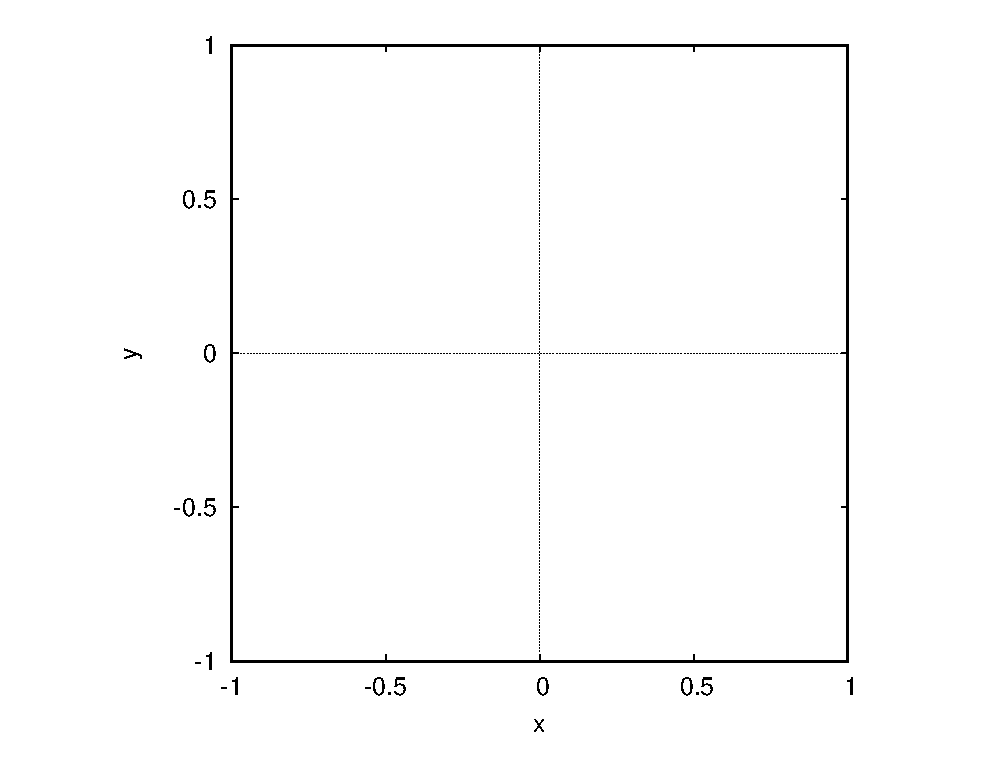
\includegraphics[width=\linewidth, height=30mm]{pic/_old_sol__0_0_1__0__10__1e2_trajectory}
        \caption{Траектория $X, Y$}
        \label{fig:_old_sol__0_0_1__0__10__1e2_trajectory}
    \end{subfigure}
    \begin{subfigure}[t]{0.3\textwidth}
        \centering
        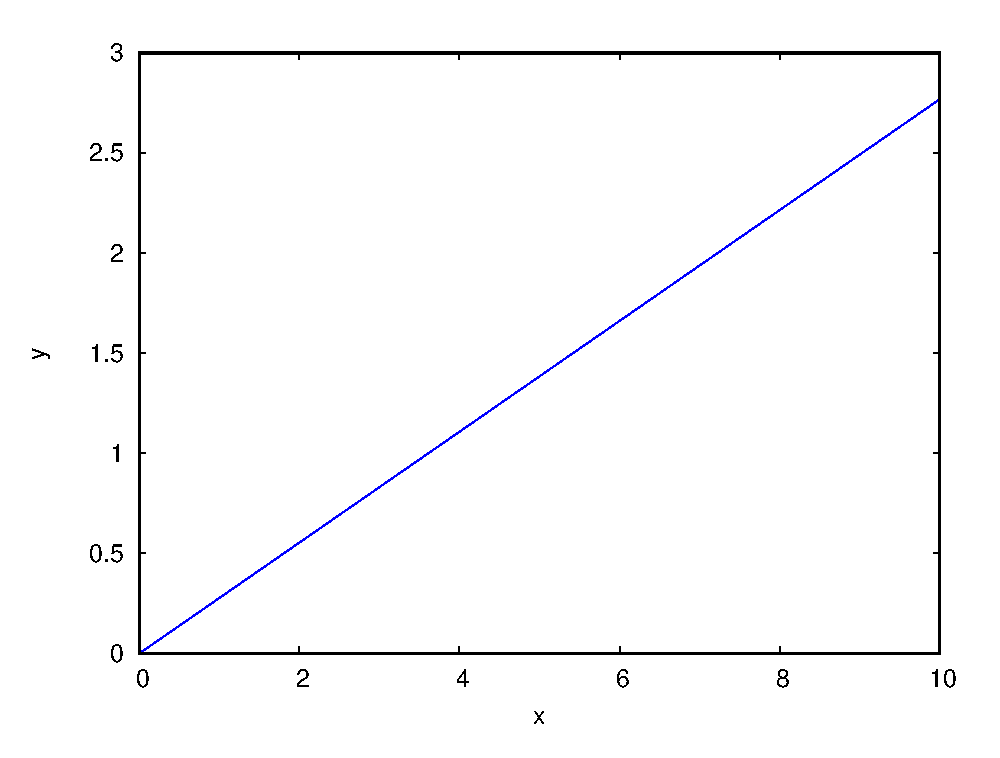
\includegraphics[width=\linewidth, height=30mm]{pic/_old_sol__0_0_1__0__10__1e2_theta}
        \caption{$\theta(t)$}
        \label{fig:_old_sol__0_0_1__0__10__1e2_theta}
    \end{subfigure}
    \vspace{12pt}
    
    \begin{subfigure}[t]{0.3\textwidth}
        \centering
        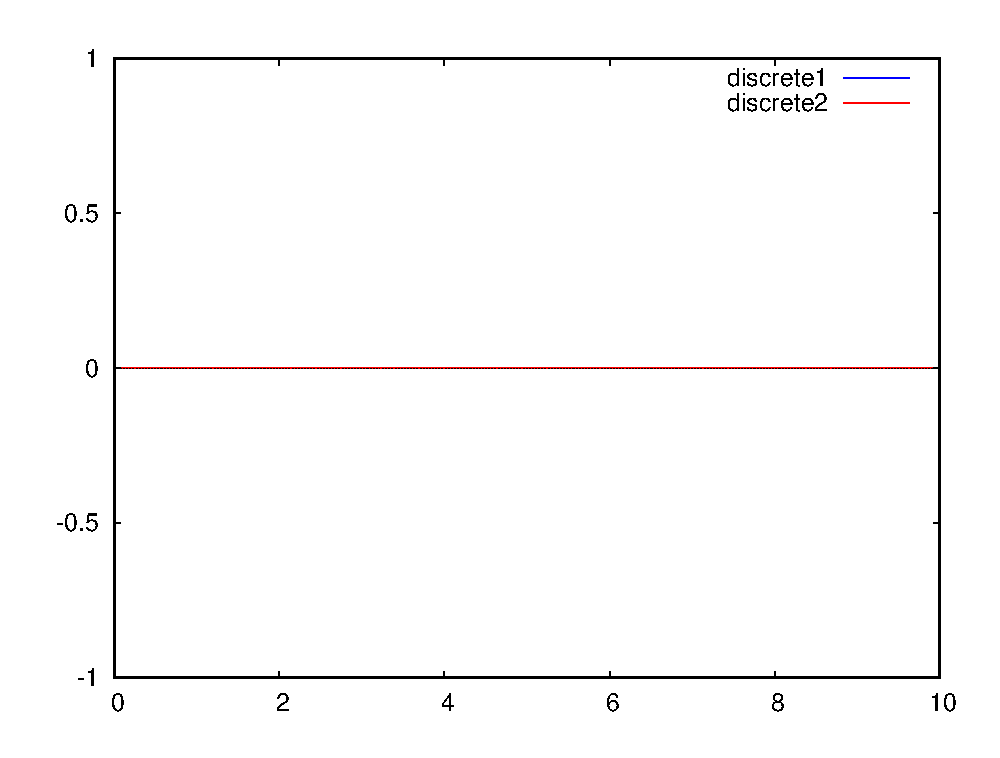
\includegraphics[width=\linewidth, height=30mm]{pic/_old_sol__0_0_1__0__10__1e2_nu12}
        \caption{$\nu_1(t), \nu_2(t)$}
        \label{fig:_old_sol__0_0_1__0__10__1e2_nu12}    
    \end{subfigure}
    \hfill
    \begin{subfigure}[t]{0.3\textwidth}
        \centering
        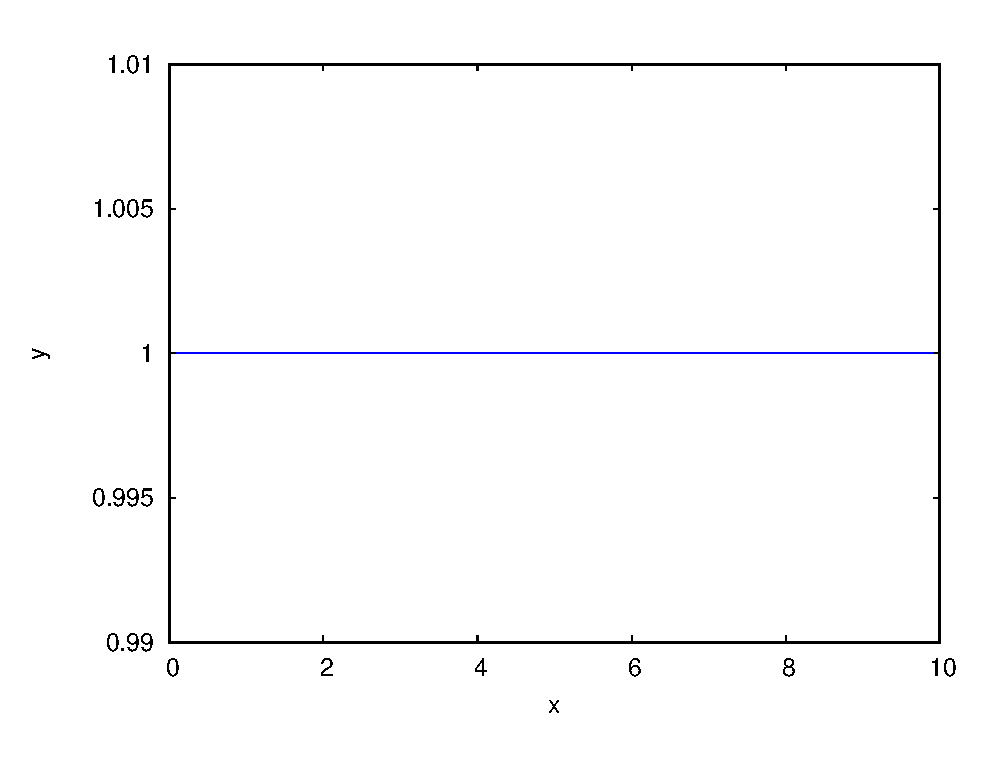
\includegraphics[width=\linewidth, height=30mm]{pic/_old_sol__0_0_1__0__10__1e2_nu3} \\
        \caption{$\nu_3(t)$}
        \label{fig:_old_sol__0_0_1__0__10__1e2_nu3}
    \end{subfigure}
    \hfill
    \begin{subfigure}[t]{0.3\textwidth}
        \centering
        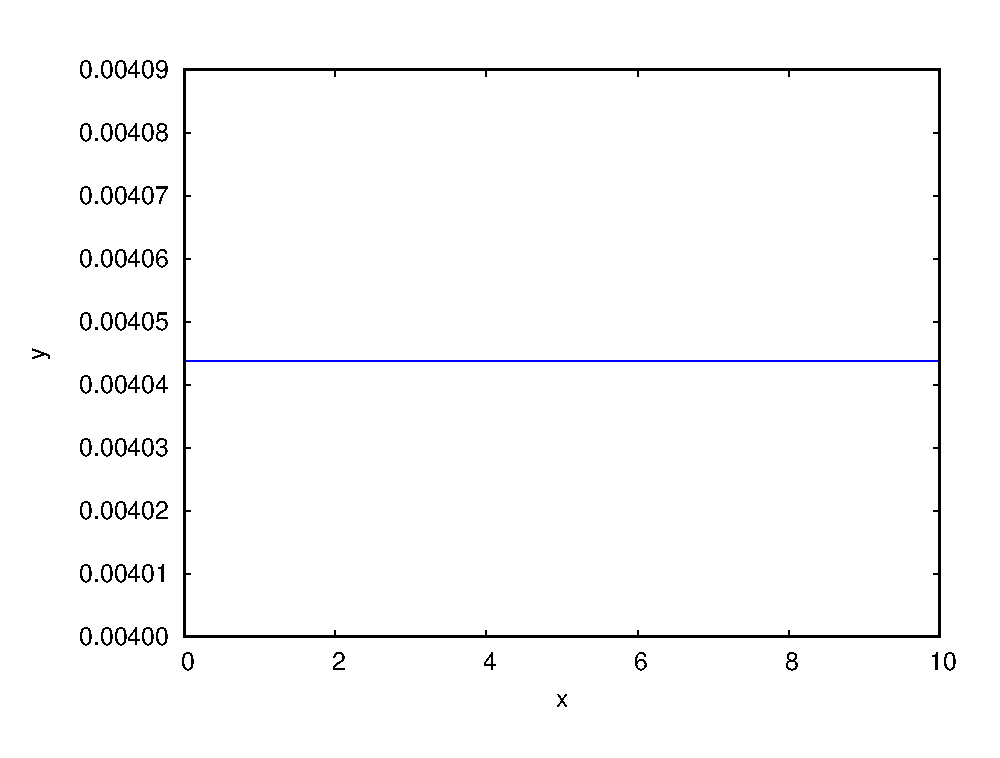
\includegraphics[width=\linewidth, height=30mm]{pic/_old_sol__0_0_1__0__10__1e2_kin_en}
        \caption{Кинетическая энергия}
        \label{fig:_old_sol__0_0_1__0__10__1e2_kin_en}
    \end{subfigure}
    
    \caption{Экипаж без роликов. Вращение вокруг своей оси ($\nu_{1,2}(0) = 0, \nu_3 = 1$). Центр экипажа неподвижен, скорость вращения и энергия постоянны.}
    \label{fig:old_selfrot}
\end{figure}

% \begin{figure}
    \centering

    % \begin{subfigure}[t]{0.3\textwidth}
    %     \centering
    %     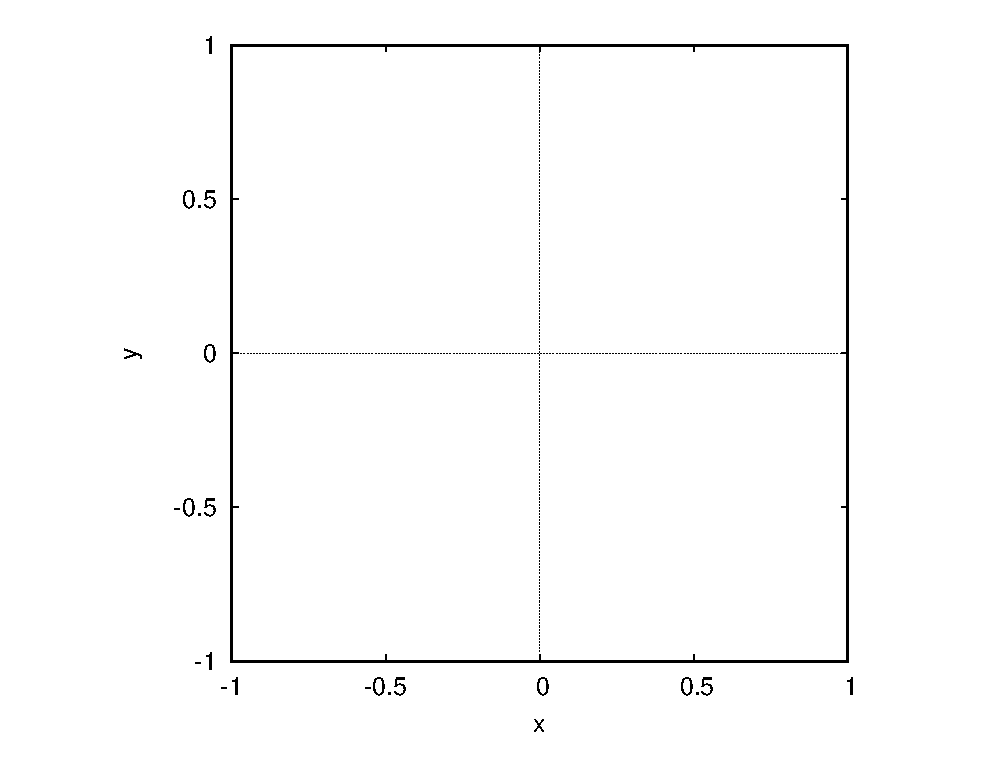
\includegraphics[width=\linewidth, height=30mm]{pic/_sol__0_0_1__0__10__1e2_trajectory}
    %     \caption{Траектория $X, Y$}
    %     \label{fig:_sol__0_0_1__0__10__1e2_trajectory}
    % \end{subfigure}
    % \begin{subfigure}[t]{0.3\textwidth}
    %     \centering
    %     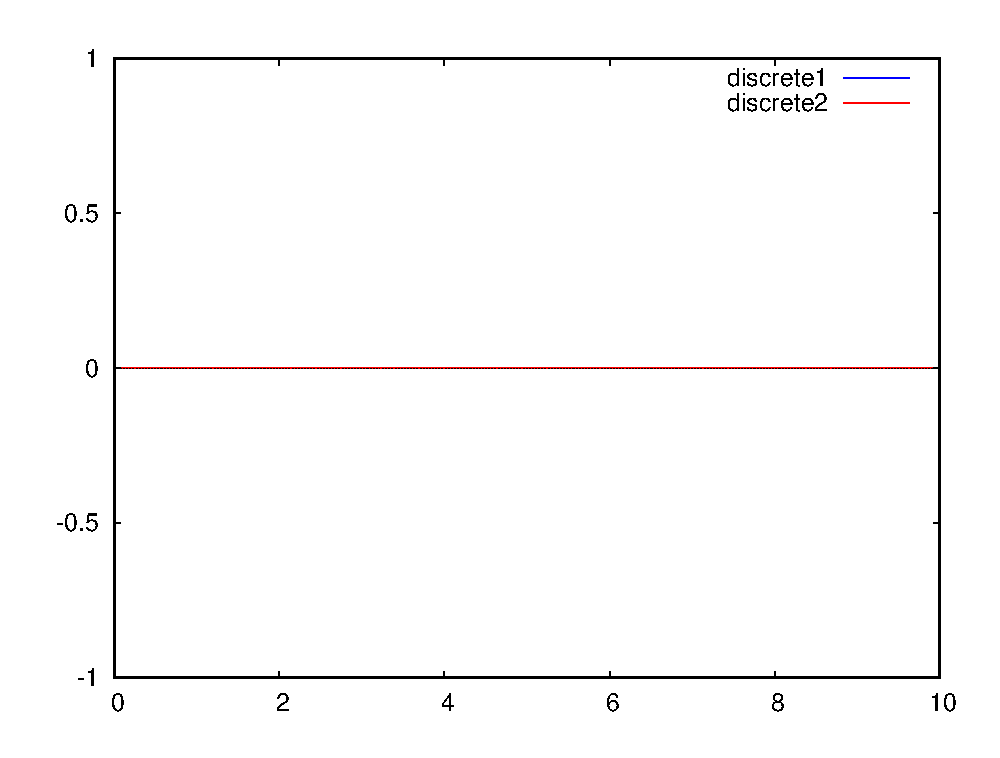
\includegraphics[width=\linewidth, height=30mm]{pic/_sol__0_0_1__0__10__1e2_nu12}
    %     \caption{$\nu_1(t), \nu_2(t)$}
    %     \label{fig:_sol__0_0_1__0__10__1e2_nu12}    
    % \end{subfigure}
    
    % \begin{subfigure}[t]{0.3\textwidth}
    %     \centering
    %     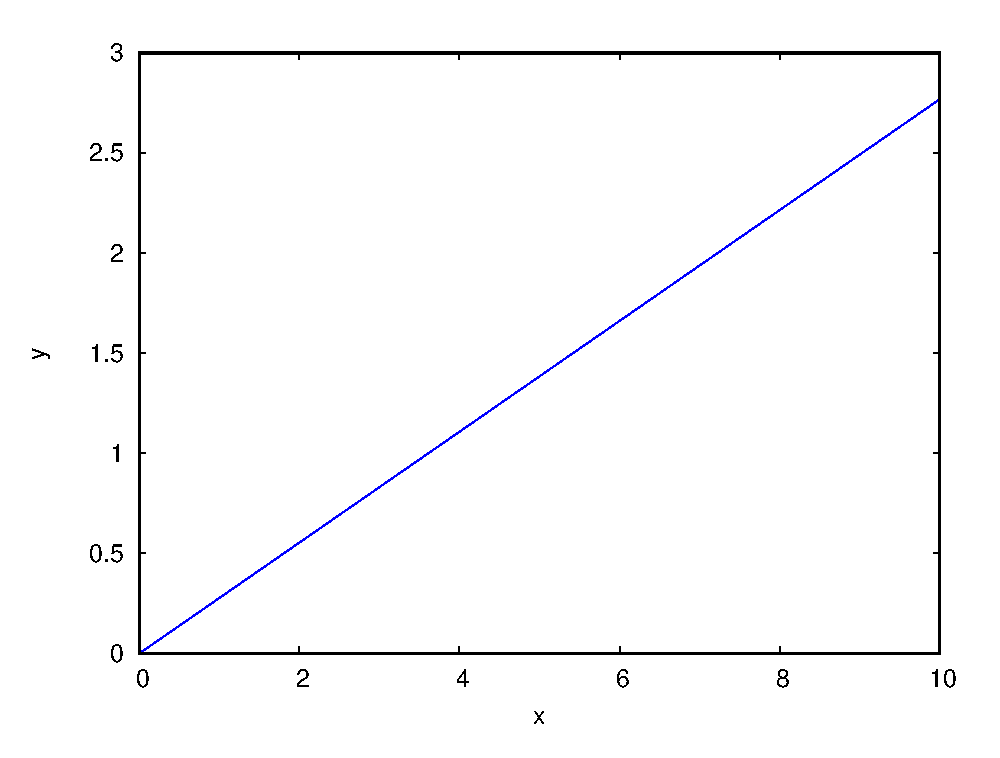
\includegraphics[width=\linewidth, height=30mm]{pic/_sol__0_0_1__0__10__1e2_theta}
    %     \caption{$\theta(t)$}
    %     \label{fig:_sol__0_0_1__0__10__1e2_theta}
    % \end{subfigure}
    % \vspace{12pt}
    
    % \begin{subfigure}[t]{0.3\textwidth}
    %     \centering
    %     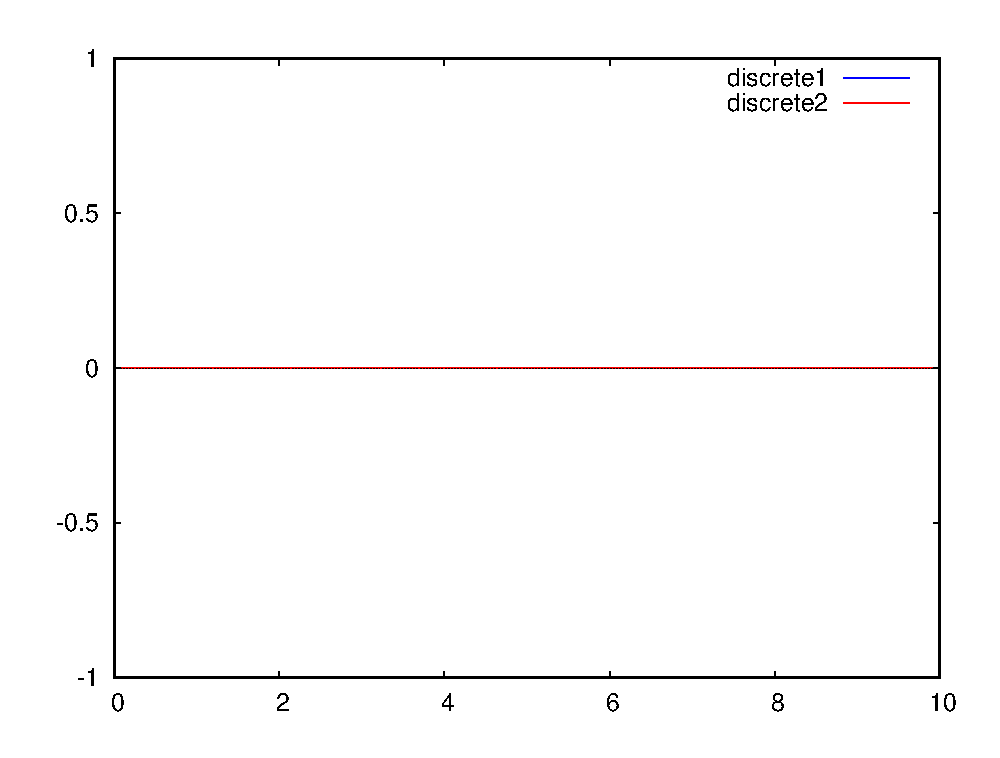
\includegraphics[width=\linewidth, height=30mm]{pic/_sol__0_0_1__0__10__1e2_nu12}
    %     \caption{$\nu_1(t), \nu_2(t)$}
    %     \label{fig:_sol__0_0_1__0__10__1e2_nu12}    
    % \end{subfigure}
    % \hfill
    % \begin{subfigure}[t]{0.3\textwidth}
    %     \centering
    %     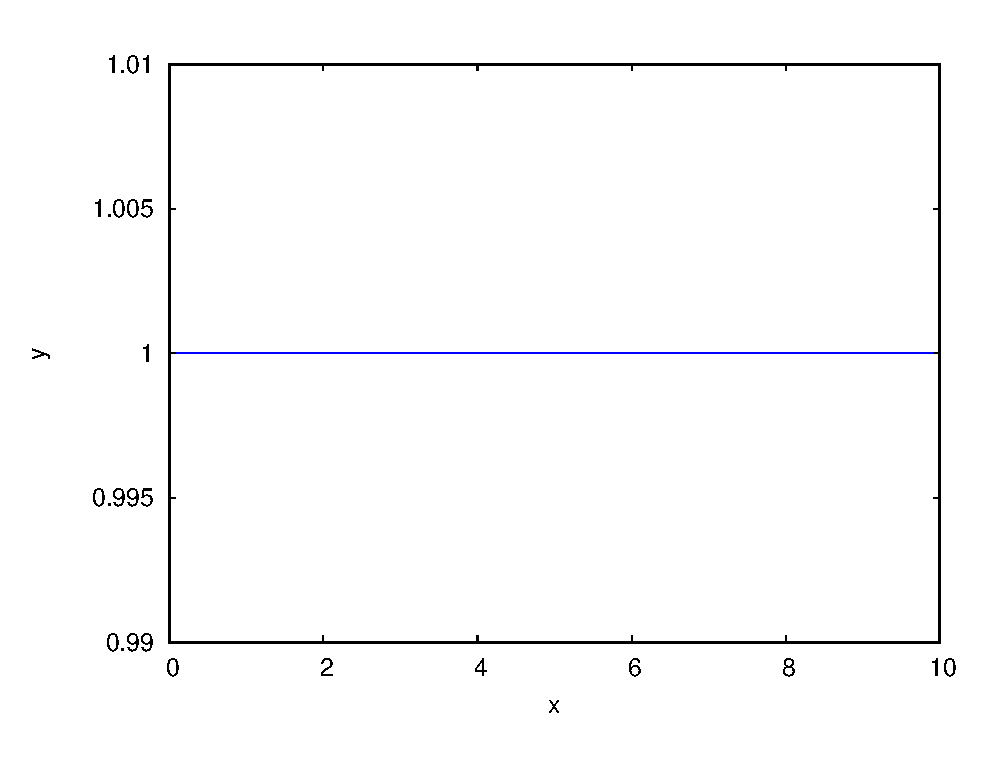
\includegraphics[width=\linewidth, height=30mm]{pic/_sol__0_0_1__0__10__1e2_nu3} \\
    %     \caption{$\nu_3(t)$}
    %     \label{fig:_sol__0_0_1__0__10__1e2_nu3}
    % \end{subfigure}
    % \hfill
    % \begin{subfigure}[t]{0.3\textwidth}
    %     \centering
    %     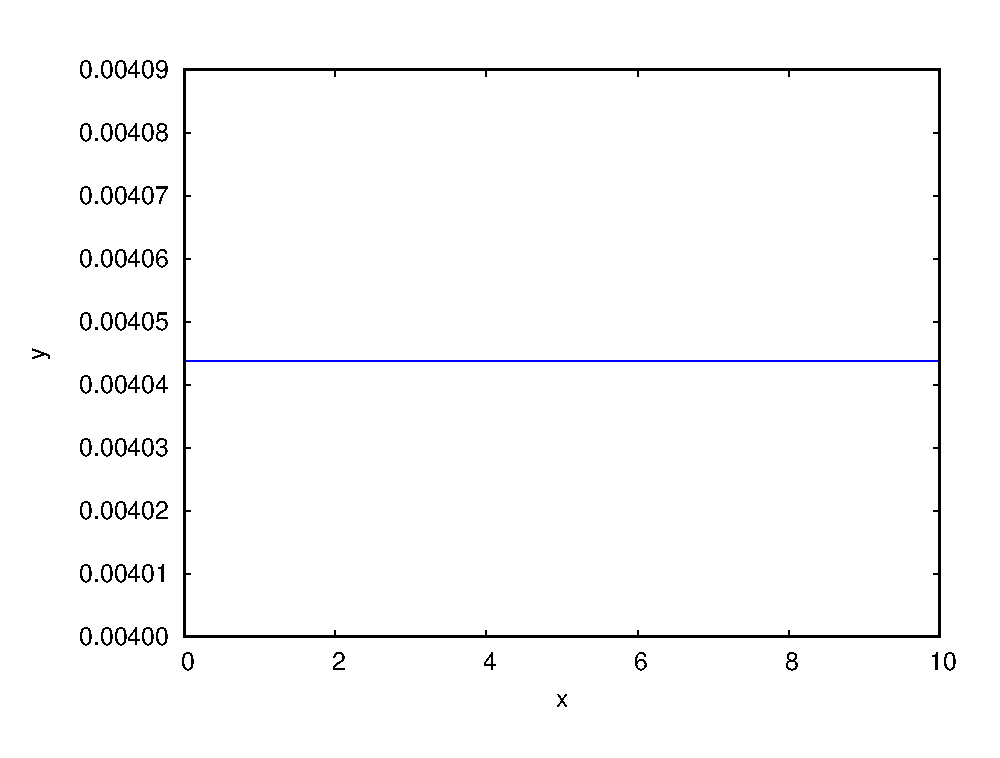
\includegraphics[width=\linewidth, height=30mm]{pic/_sol__0_0_1__0__10__1e2_kin_en}
    %     \caption{Кинетическая энергия}
    %     \label{fig:_sol__0_0_1__0__10__1e2_kin_en}
    % \end{subfigure}
    
    \begin{subfigure}[t]{0.3\textwidth}
        \centering
        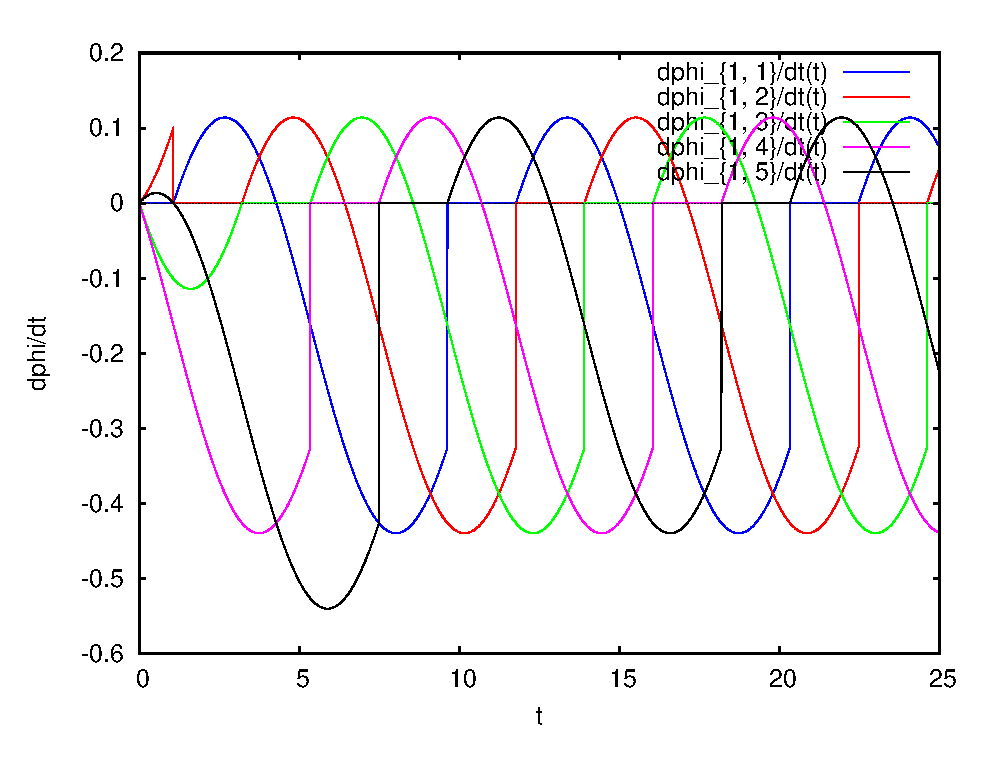
\includegraphics[width=\linewidth]{pic/rol__self_rot__velocities_of_rollers_of_wheel_1}
        \caption{Скорости роликов $\dot{\phi}_{ij}(t)$ на любом колесе}
        \label{fig:rol__self_rot__velocities_of_rollers_of_wheel_1}
    \end{subfigure}
    \begin{subfigure}[t]{0.3\textwidth}
        \centering
        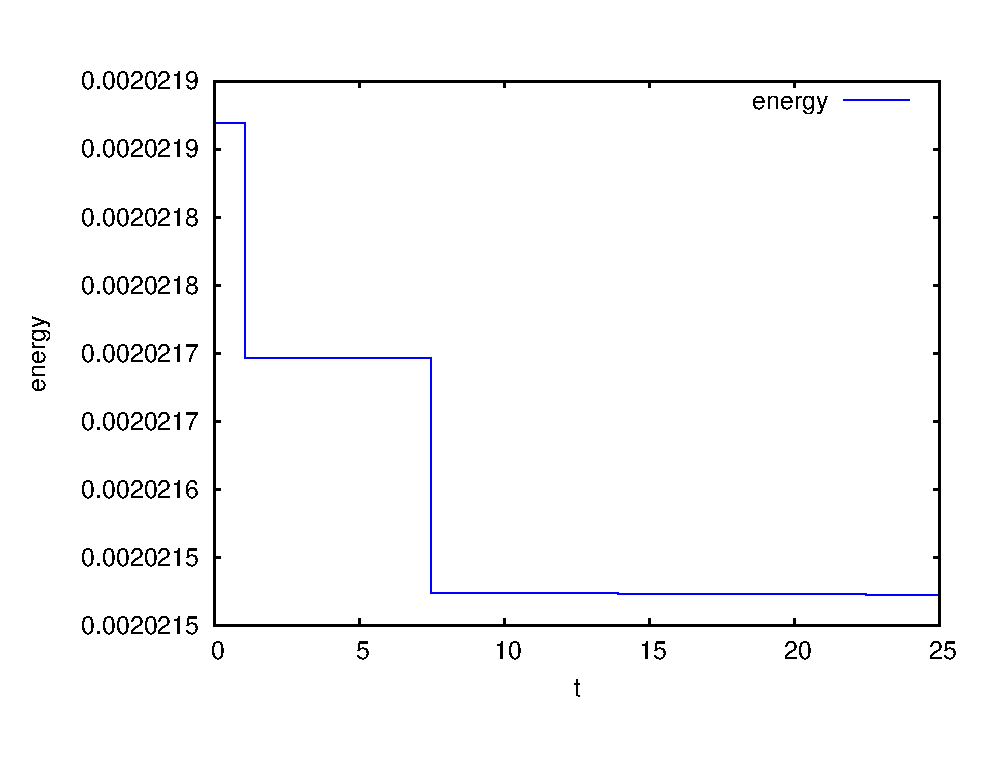
\includegraphics[width=\linewidth]{pic/rol__self_rot__kinetic_energy}
        \caption{Кинетическая энергия}
        \label{fig:rol__self_rot__kinetic_energy}    
    \end{subfigure}
    \begin{subfigure}[t]{0.3\textwidth}
        \centering
        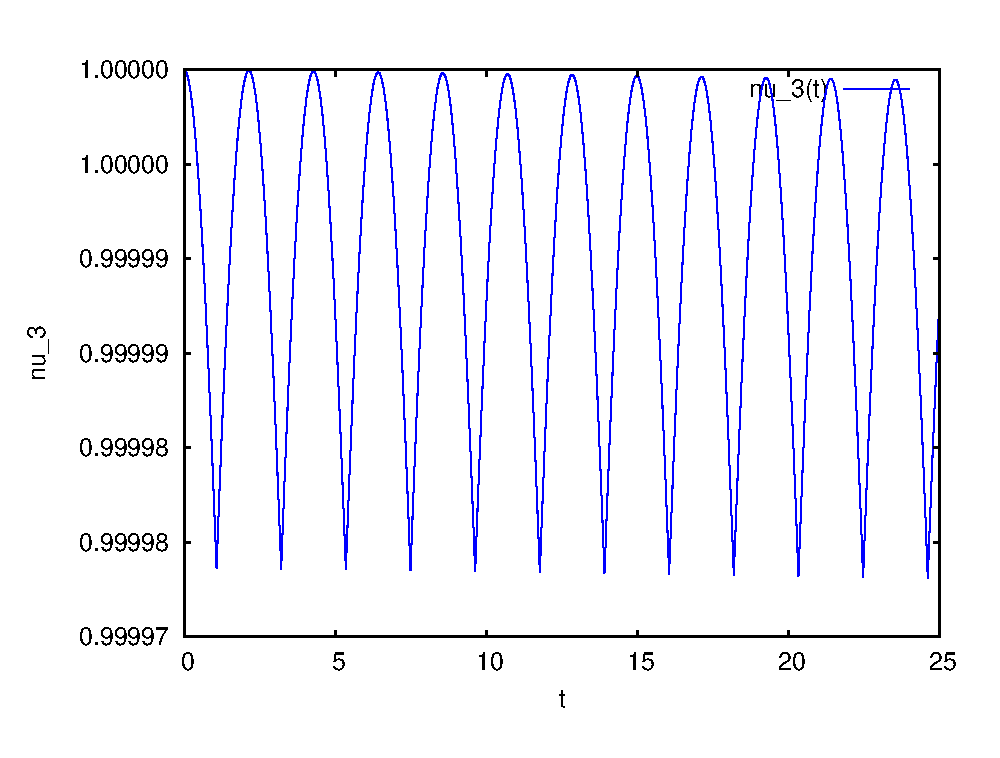
\includegraphics[width=\linewidth]{pic/rol__self_rot__velocity_of_self_rotation}
        \caption{Угловая скорость собственного вращения $\nu_3(t)$}
        \label{fig:rol__self_rot__velocity_of_self_rotation}    
    \end{subfigure}

    \caption{Экипаж с роликами. Вращение вокруг своей оси ($\nu_{1,2}(0) = 0, \nu_3 = 1$).}
    \label{fig:selfrot}
    
\end{figure}


% \begin{figure}
    \centering
    \begin{subfigure}[t]{0.3\textwidth}
        \centering
        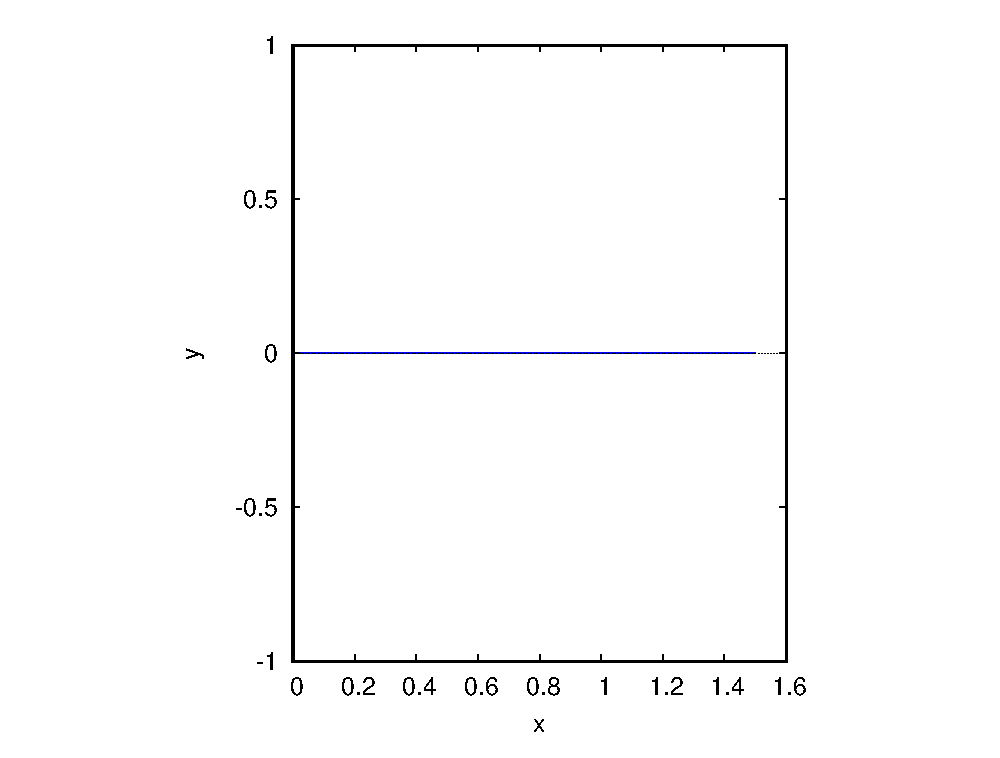
\includegraphics[width=\linewidth, height=30mm]{pic/_old_sol__1_0_0__0__10__1e2_trajectory}
        \caption{Траектория $X, Y$}
        \label{fig:_old_sol__1_0_0__0__10__1e2_trajectory}
    \end{subfigure}
    \begin{subfigure}[t]{0.3\textwidth}
        \centering
        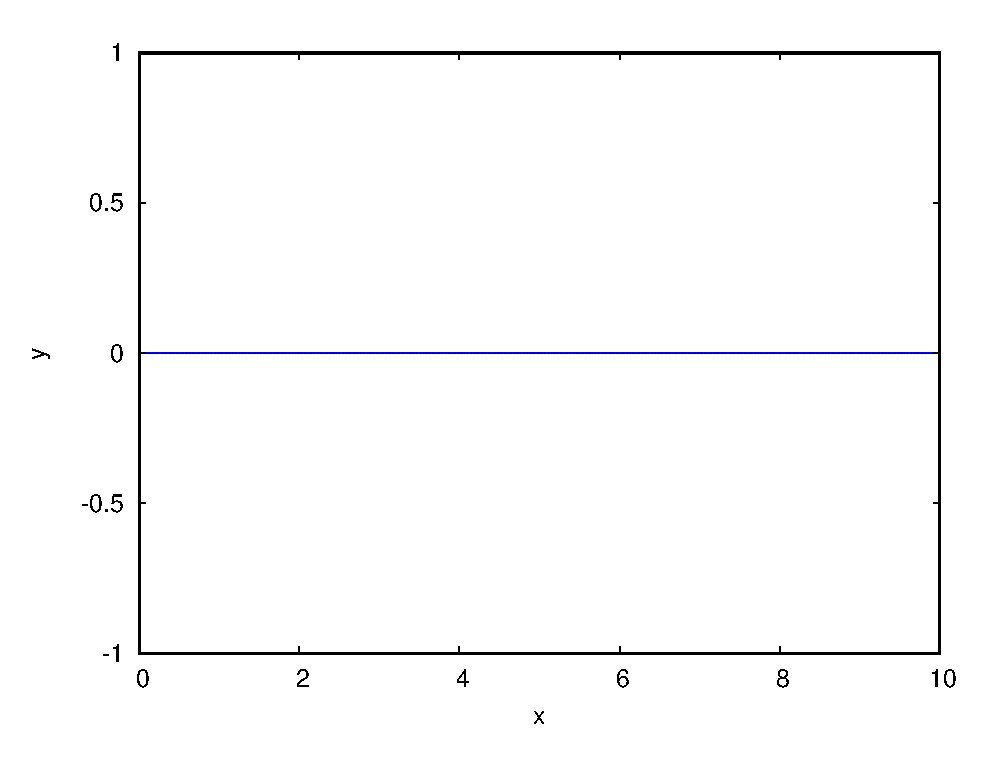
\includegraphics[width=\linewidth, height=30mm]{pic/_old_sol__1_0_0__0__10__1e2_theta}
        \caption{$\theta(t)$}
        \label{fig:_old_sol__1_0_0__0__10__1e2_theta}
    \end{subfigure}
    \vspace{12pt}
    
    \begin{subfigure}[t]{0.3\textwidth}
        \centering
        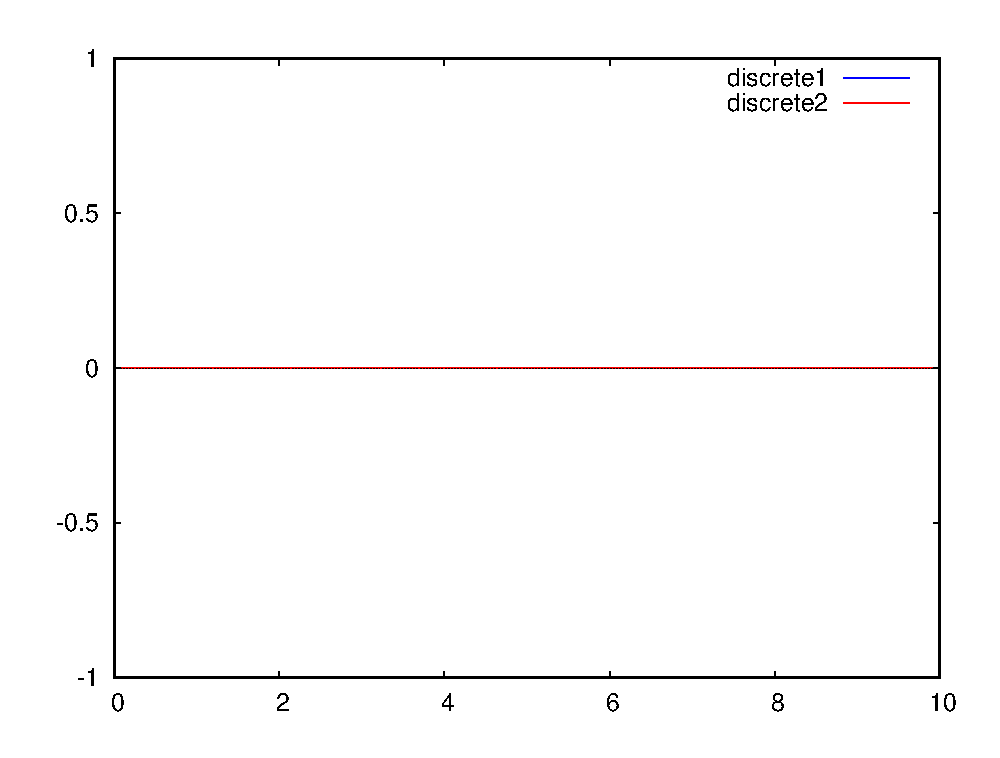
\includegraphics[width=\linewidth, height=30mm]{pic/_old_sol__1_0_0__0__10__1e2_nu12_centered}
        \caption{$\nu_1(t), \nu_2(t)$}
        \label{fig:_old_sol__1_0_0__0__10__1e2_nu12_centered}    
    \end{subfigure}
    \hfill
    \begin{subfigure}[t]{0.3\textwidth}
        \centering
        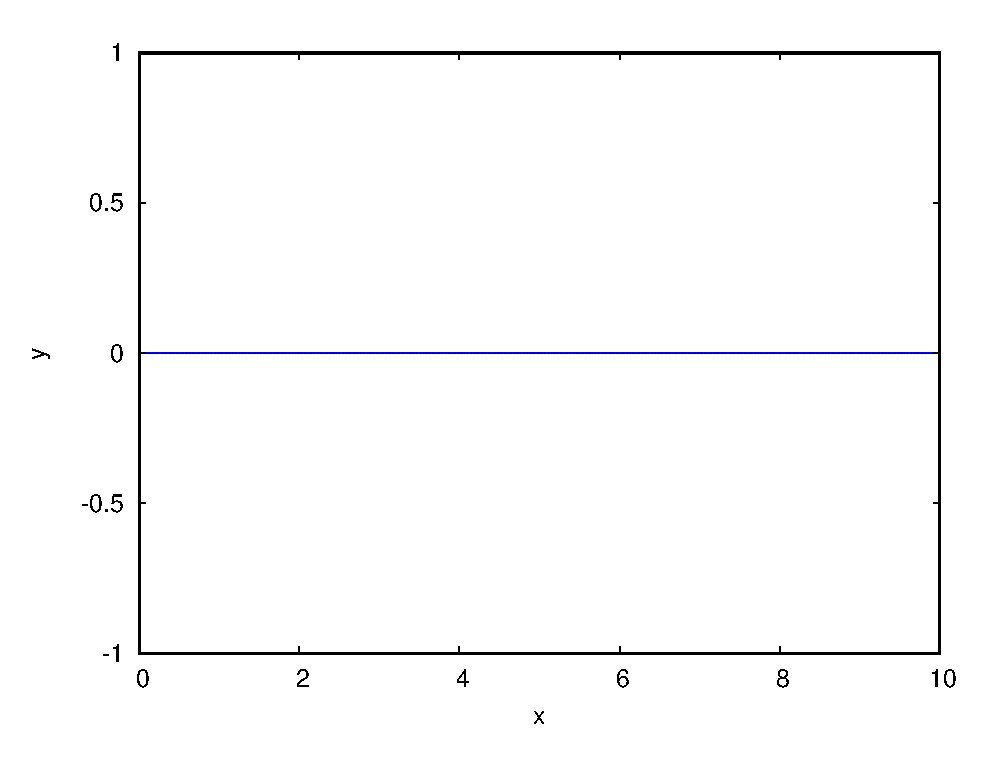
\includegraphics[width=\linewidth, height=30mm]{pic/_old_sol__1_0_0__0__10__1e2_nu3} \\
        \caption{$\nu_3(t)$}
        \label{fig:_old_sol__1_0_0__0__10__1e2_nu3}
    \end{subfigure}
    \hfill
    \begin{subfigure}[t]{0.3\textwidth}
        \centering
        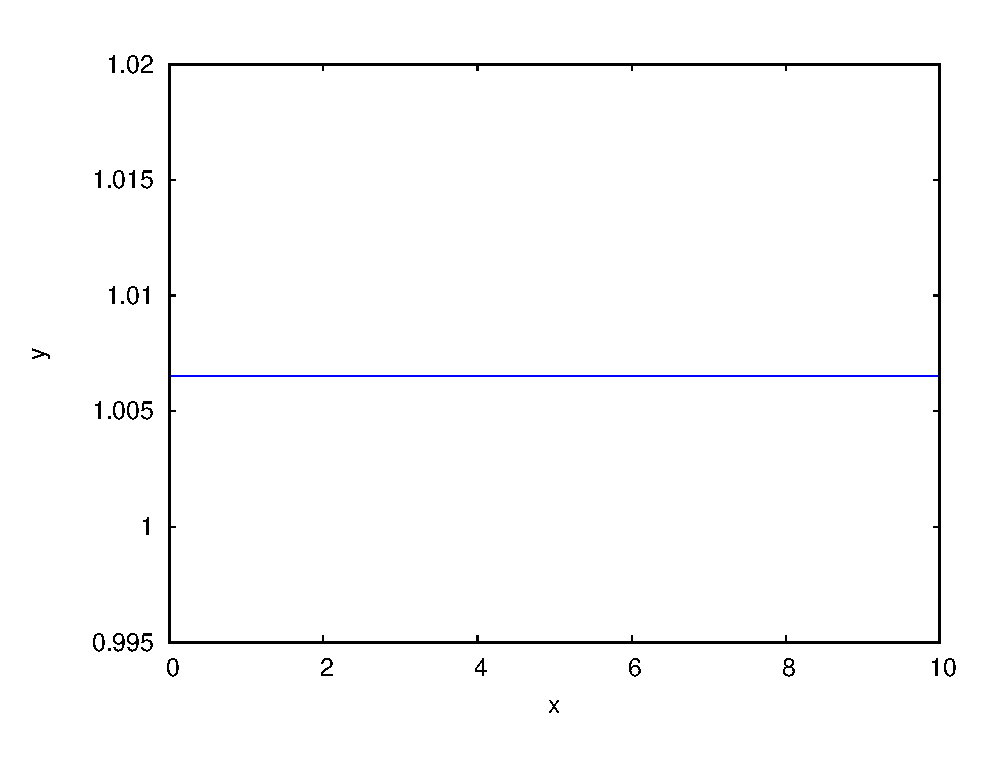
\includegraphics[width=\linewidth, height=30mm]{pic/_old_sol__1_0_0__0__10__1e2_kin_en}
        \caption{Кинетическая энергия}
        \label{fig:_old_sol__1_0_0__0__10__1e2_kin_en}
    \end{subfigure}
    
    \caption{Экипаж без роликов. Движение по прямой ($\nu_1(0) = 1, \nu_{2,3} = 0$). Экипаж равномерно движется по прямой, не вращаясь, энергия постоянна.}
    \label{fig:old_straight}
\end{figure}


% \begin{figure}[H]
    \centering

    \begin{columns}
        \column{0.45\textwidth}
            \centering
            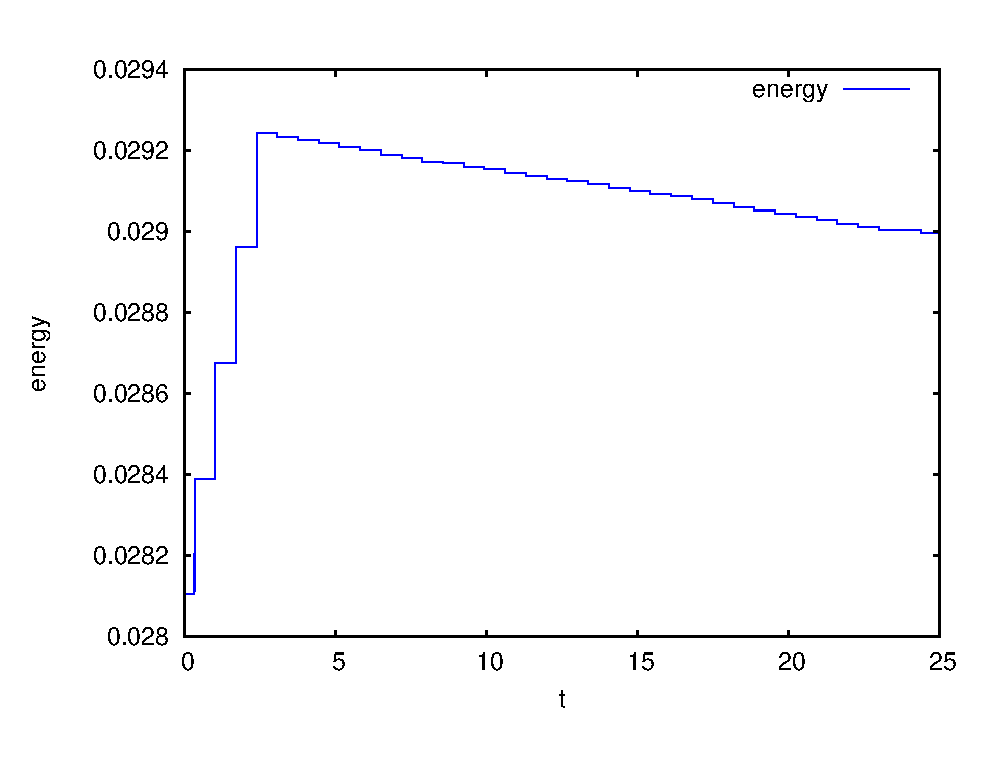
\includegraphics[width=\linewidth]{pic/rol__straight__kinetic_energy}\\
            Кинетическая энергия
        \column{0.45\textwidth}
            \centering
            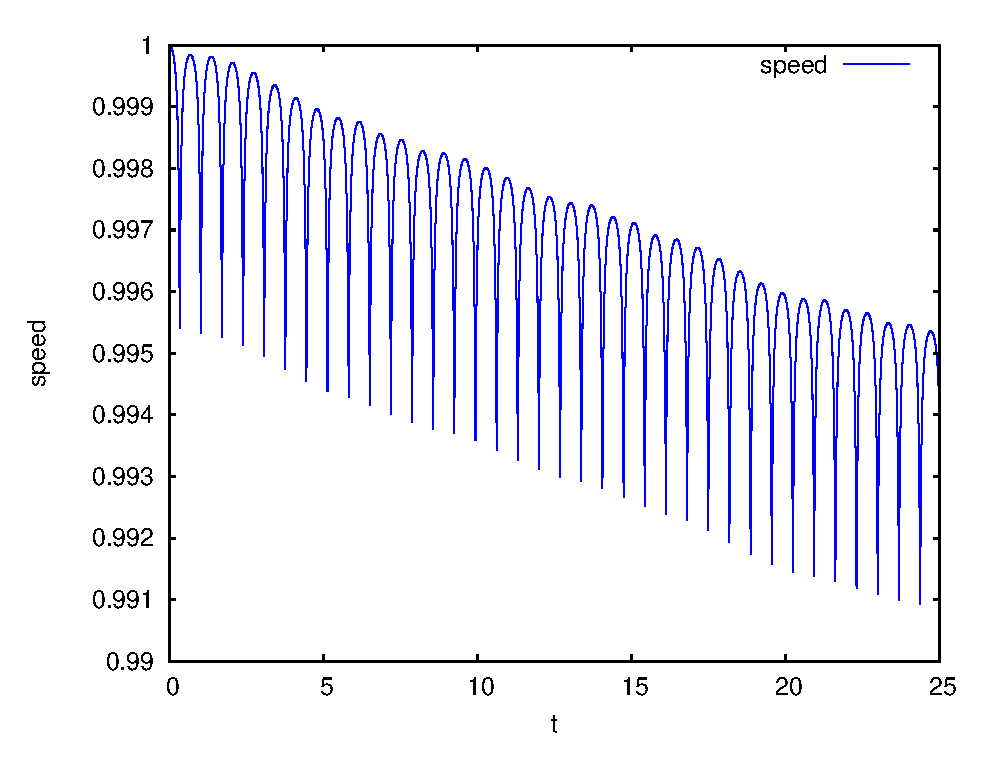
\includegraphics[width=\linewidth]{pic/rol__straight__speed_of_center_of_mass}\\
            Скорость центра масс
    \end{columns}
    
    \begin{columns}
        \column{0.35\textwidth}
            \centering
            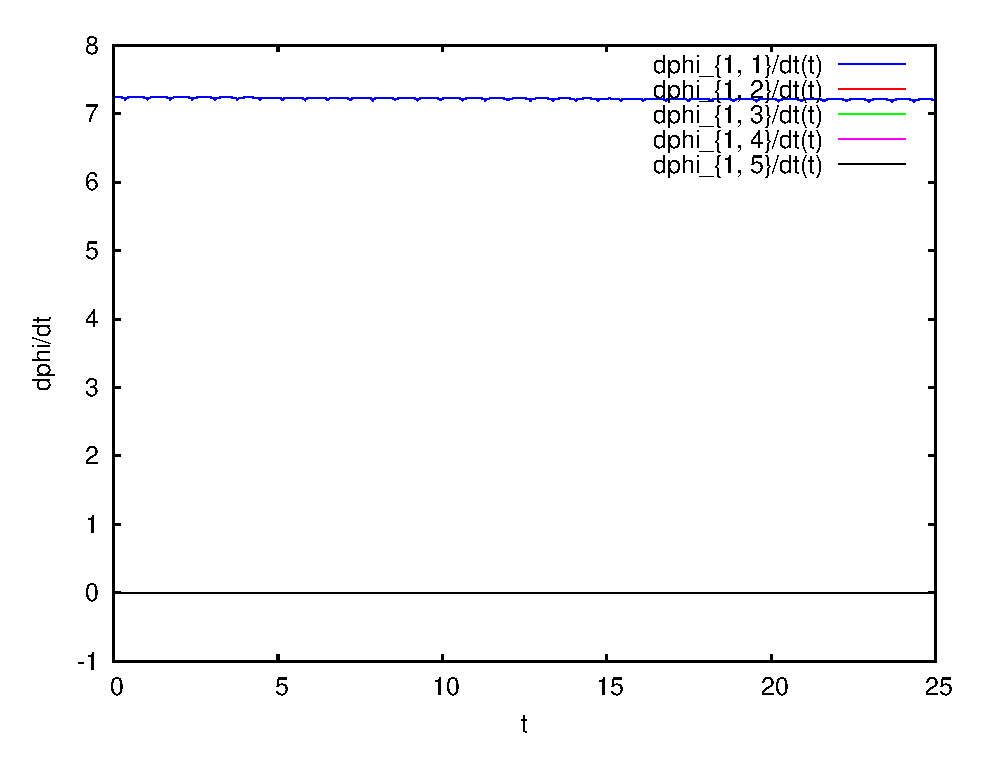
\includegraphics[width=\linewidth]{pic/rol__straight__velocities_of_rollers_of_wheel_1}\\
            $\dot{\phi}_{ij}(t)$ на переднем колесе
        \column{0.45\textwidth}
            \centering
            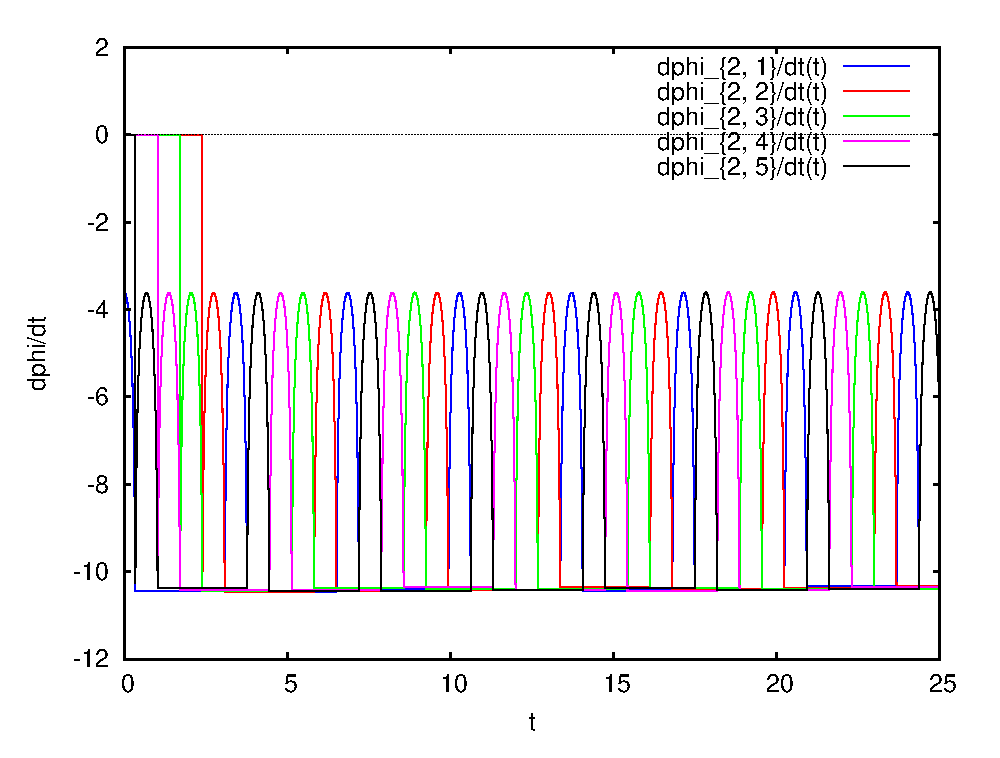
\includegraphics[width=\linewidth]{pic/rol__straight__velocities_of_rollers_of_wheel_2}\\
            $\dot{\phi}_{ij}(t)$ на правом заднем колесе
    \end{columns}

\end{figure}


%\section{Результаты расчетов}

\newpage

{\bf Фигуры.}
\stepcounter{section}

\begin{figure}[H]
    \hspace{-0.6cm}
    % \minipage{0.5\textwidth}
        % \centering
        \scalebox{1.5}{\asyinclude{./asy/pic_wheel.asy}}
        %\caption{Колесо}
        % \caption{\ }
        % \label{fig:wheel}
    % \endminipage
    \quad
    % \minipage{0.55\textwidth}
        % \centering
        \scalebox{1.5}{\asyinclude{./asy/pic_cart.asy}}
        %\caption{Экипаж}
        \caption{\ }
        % \label{fig:vehicle}
        \label{fig:wheel}
    % \endminipage
\end{figure}

\begin{figure}[H]
    \centering
    \scalebox{1.5}{\asyinclude{./asy/pic_overlap.asy}}
    \quad
    \scalebox{1.5}{\asyinclude{./asy/pic_change.asy}}
    \caption{\ }
    \label{fig:overlap_and_change}
\end{figure}



\begin{figure}[H]
  \hspace{2.73cm}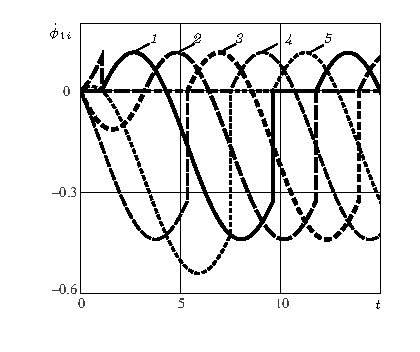
\includegraphics[width=0.6\textwidth]{pic/figure5_1.pdf}
  \caption{\ }
  %\caption{Угловые скорости роликов колеса при вращении экипажа вокруг вертикали}
  \label{fig:selfrot}
\end{figure}

\begin{figure}[H]
  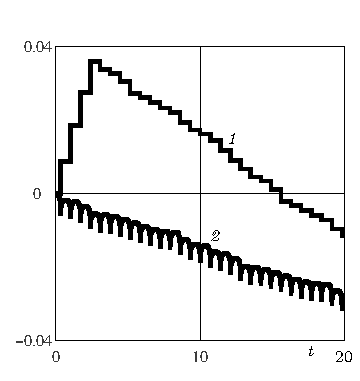
\includegraphics[width=0.45\textwidth]{pic/figure6_1.pdf}
  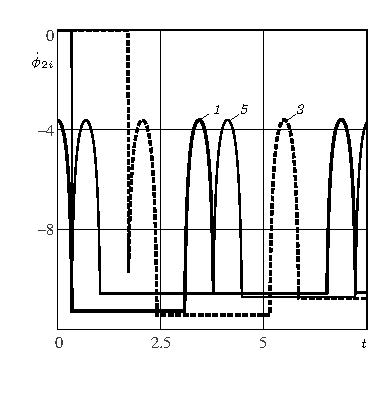
\includegraphics[width=0.45\textwidth]{pic/figure6_2.pdf}
  %\caption{Изменение энергии и скорости центра масс (слева) и угловые скорости роликов бокового колеса (справа) при прямолинейном движении}
  \caption{\ }
  \label{fig:straight}
\end{figure}

\begin{figure}[H]
  \hspace{-1.4cm}
  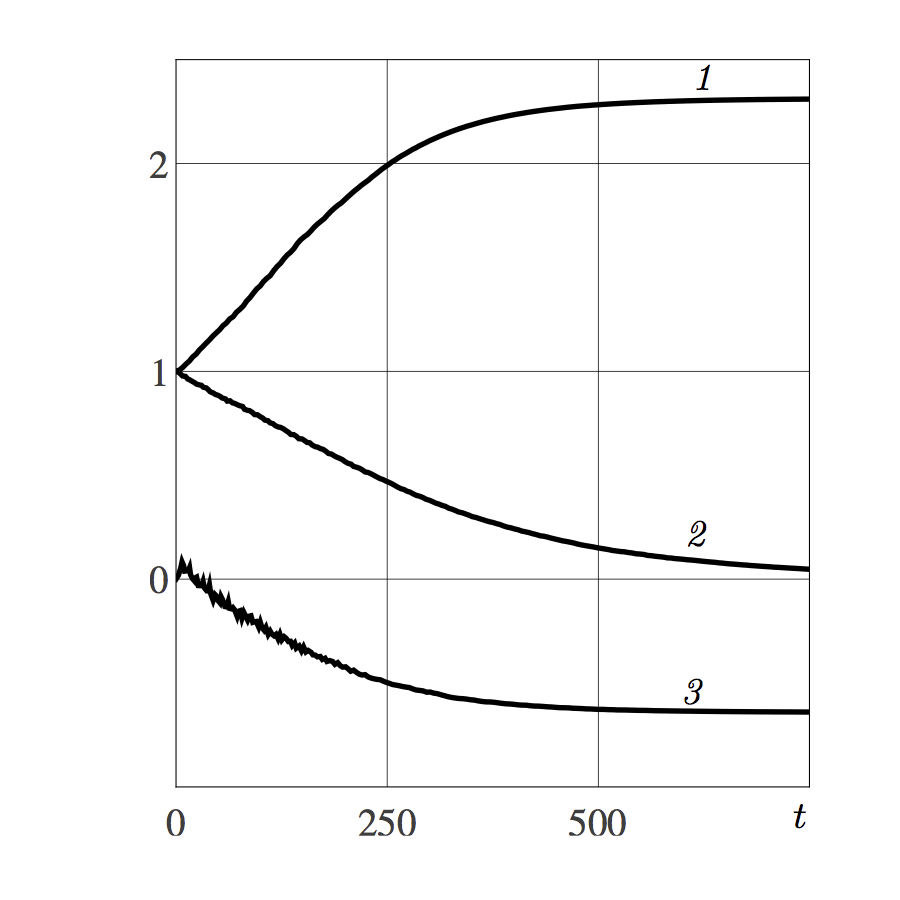
\includegraphics[width=0.5\textwidth]{pic/figure7_1.png}
  \hspace{-0.7cm}
  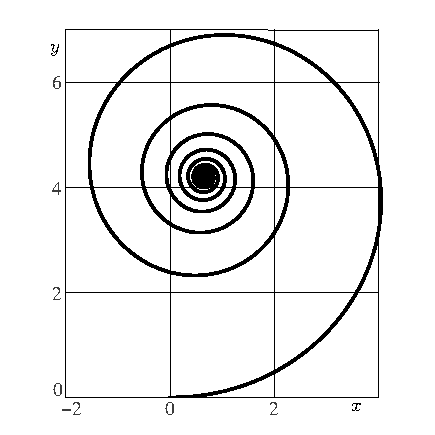
\includegraphics[width=0.65\textwidth]{pic/figure7_3.pdf}
  \begin{center}
  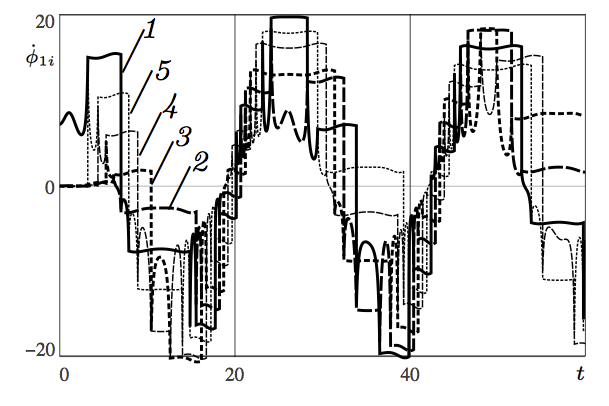
\includegraphics[width=0.8\textwidth]{pic/figure7_2.png}
  \end{center}
  %\caption{Угловая скорость, скорость центра масс и изменение энергии (вверху слева), угловые скорости роликов первого колеса (вверху справа) и траектория центра масс (внизу) при поступательно-вращательном движении}
  \caption{\ }
  \label{fig:wrench}
\end{figure}


%\begin{figure}
    \centering

    % \begin{subfigure}[t]{0.3\textwidth}
    %     \centering
    %     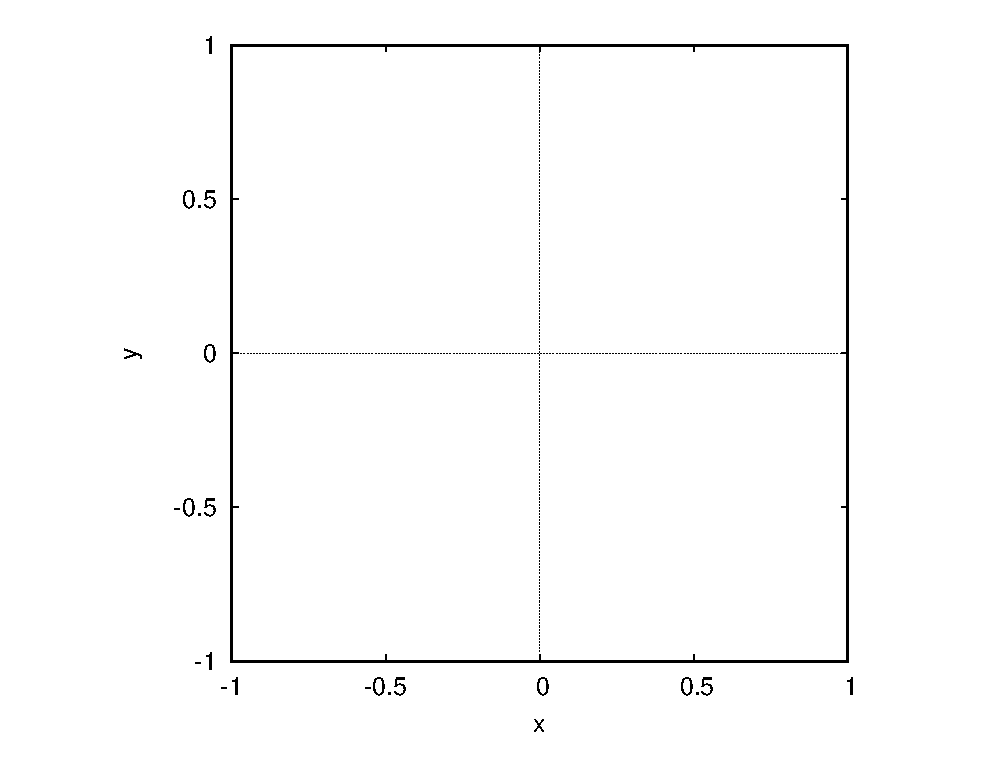
\includegraphics[width=\linewidth, height=30mm]{pic/_sol__0_0_1__0__10__1e2_trajectory}
    %     \caption{Траектория $X, Y$}
    %     \label{fig:_sol__0_0_1__0__10__1e2_trajectory}
    % \end{subfigure}
    % \begin{subfigure}[t]{0.3\textwidth}
    %     \centering
    %     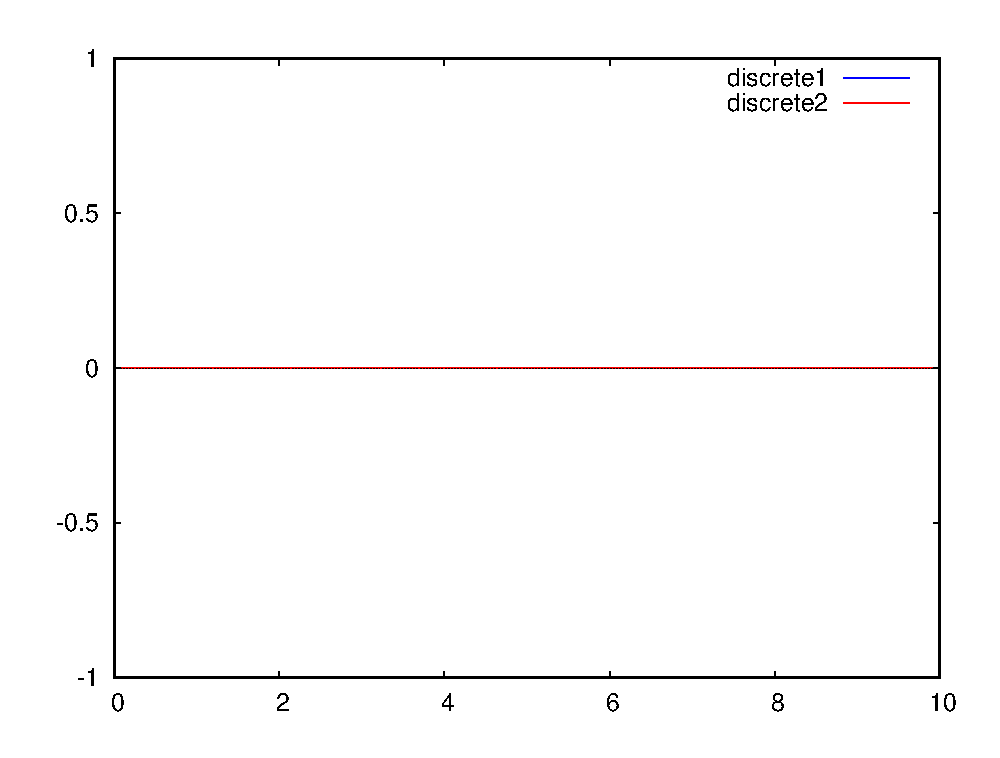
\includegraphics[width=\linewidth, height=30mm]{pic/_sol__0_0_1__0__10__1e2_nu12}
    %     \caption{$\nu_1(t), \nu_2(t)$}
    %     \label{fig:_sol__0_0_1__0__10__1e2_nu12}    
    % \end{subfigure}
    
    % \begin{subfigure}[t]{0.3\textwidth}
    %     \centering
    %     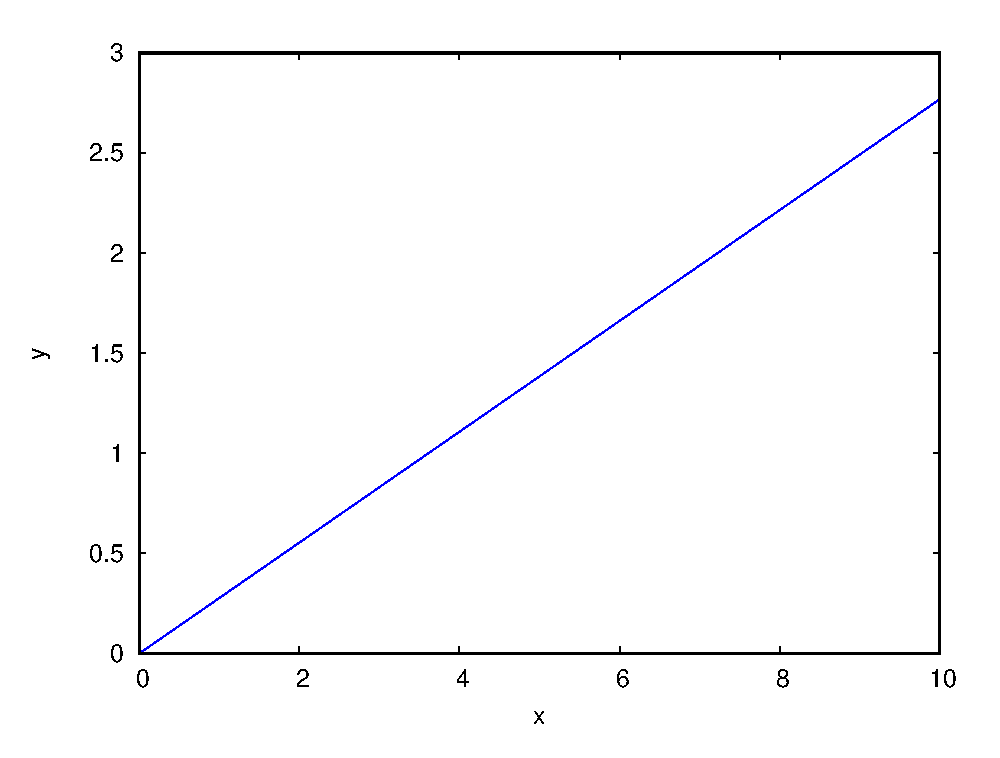
\includegraphics[width=\linewidth, height=30mm]{pic/_sol__0_0_1__0__10__1e2_theta}
    %     \caption{$\theta(t)$}
    %     \label{fig:_sol__0_0_1__0__10__1e2_theta}
    % \end{subfigure}
    % \vspace{12pt}
    
    % \begin{subfigure}[t]{0.3\textwidth}
    %     \centering
    %     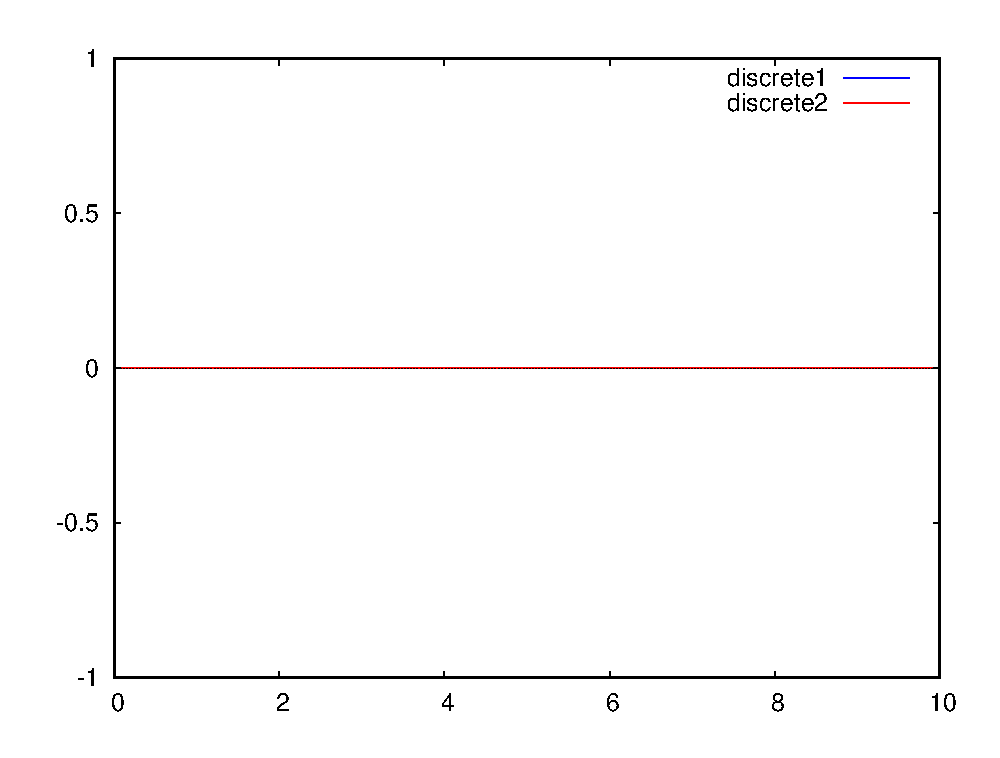
\includegraphics[width=\linewidth, height=30mm]{pic/_sol__0_0_1__0__10__1e2_nu12}
    %     \caption{$\nu_1(t), \nu_2(t)$}
    %     \label{fig:_sol__0_0_1__0__10__1e2_nu12}    
    % \end{subfigure}
    % \hfill
    % \begin{subfigure}[t]{0.3\textwidth}
    %     \centering
    %     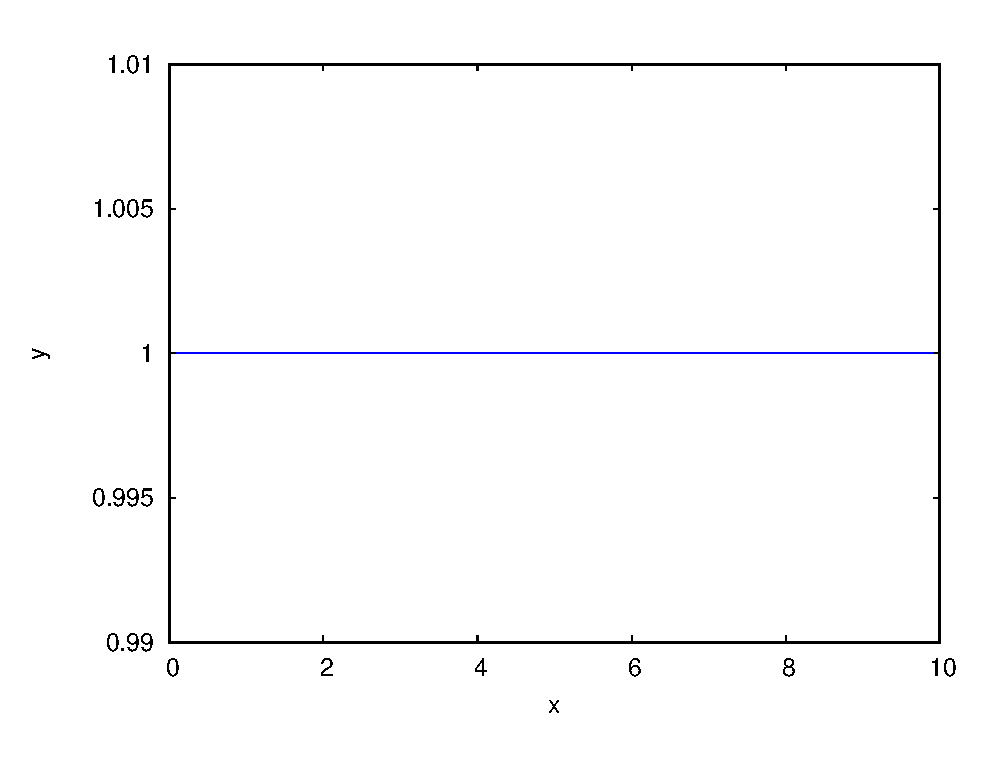
\includegraphics[width=\linewidth, height=30mm]{pic/_sol__0_0_1__0__10__1e2_nu3} \\
    %     \caption{$\nu_3(t)$}
    %     \label{fig:_sol__0_0_1__0__10__1e2_nu3}
    % \end{subfigure}
    % \hfill
    % \begin{subfigure}[t]{0.3\textwidth}
    %     \centering
    %     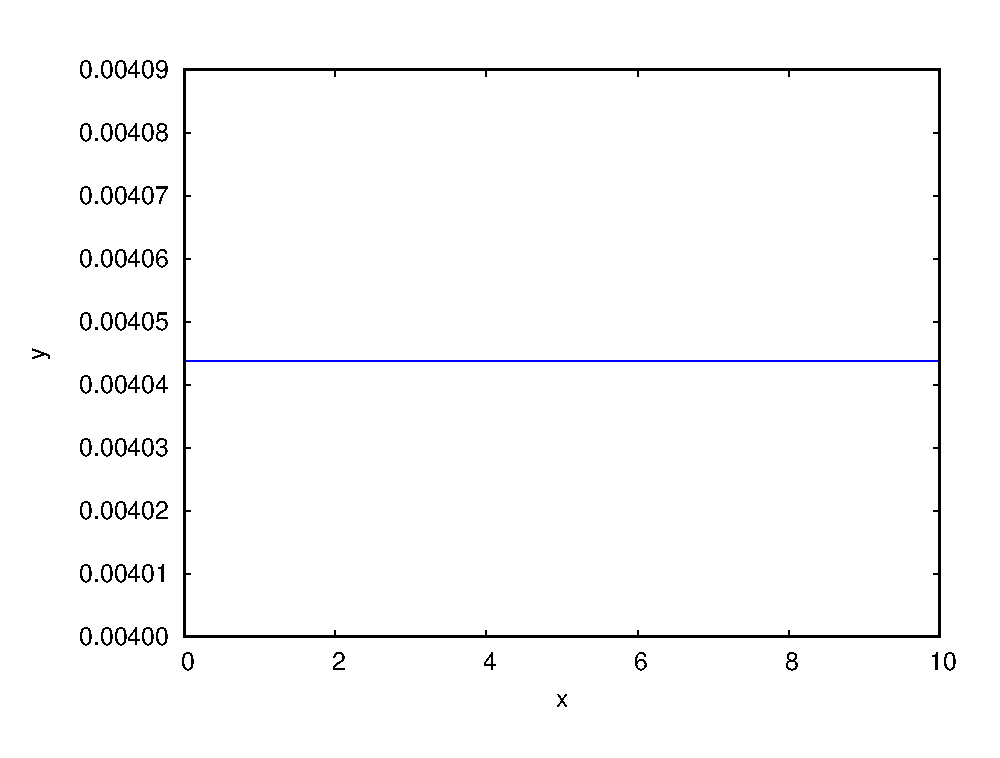
\includegraphics[width=\linewidth, height=30mm]{pic/_sol__0_0_1__0__10__1e2_kin_en}
    %     \caption{Кинетическая энергия}
    %     \label{fig:_sol__0_0_1__0__10__1e2_kin_en}
    % \end{subfigure}
    
    \begin{subfigure}[t]{0.3\textwidth}
        \centering
        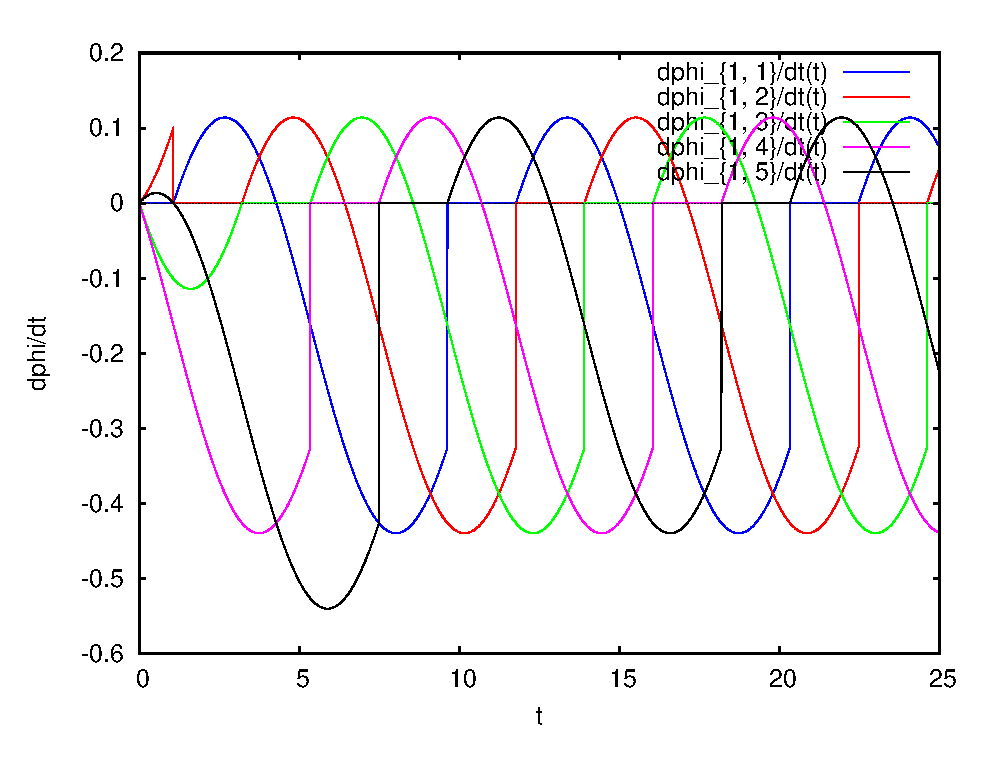
\includegraphics[width=\linewidth]{pic/rol__self_rot__velocities_of_rollers_of_wheel_1}
        \caption{Скорости роликов $\dot{\phi}_{ij}(t)$ на любом колесе}
        \label{fig:rol__self_rot__velocities_of_rollers_of_wheel_1}
    \end{subfigure}
    \begin{subfigure}[t]{0.3\textwidth}
        \centering
        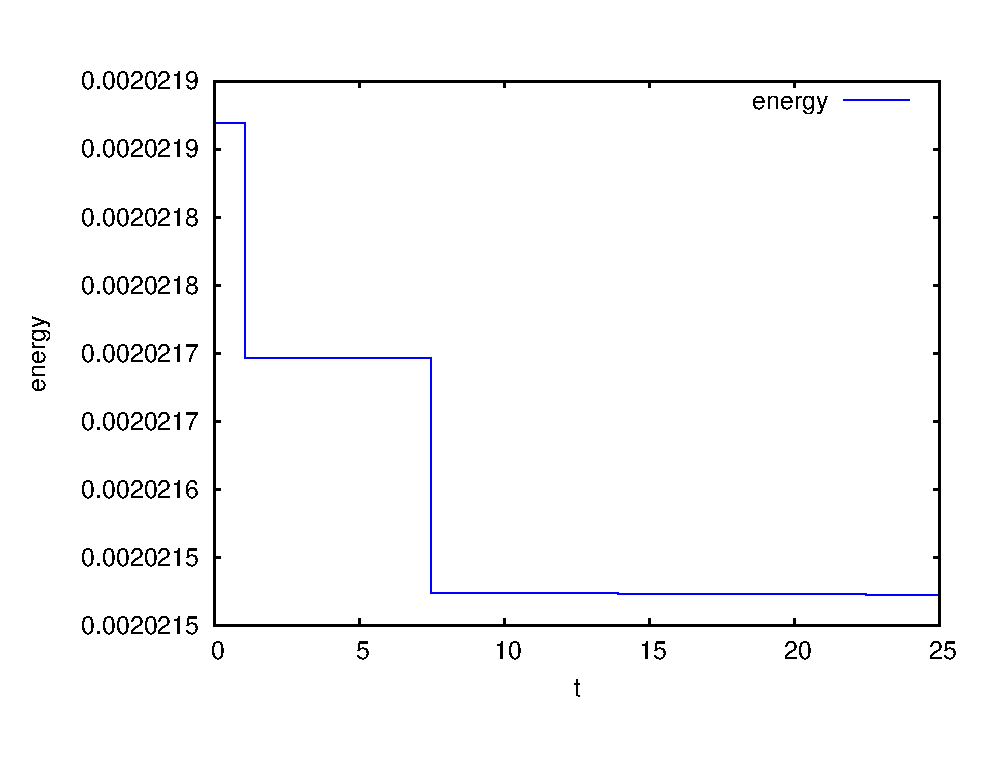
\includegraphics[width=\linewidth]{pic/rol__self_rot__kinetic_energy}
        \caption{Кинетическая энергия}
        \label{fig:rol__self_rot__kinetic_energy}    
    \end{subfigure}
    \begin{subfigure}[t]{0.3\textwidth}
        \centering
        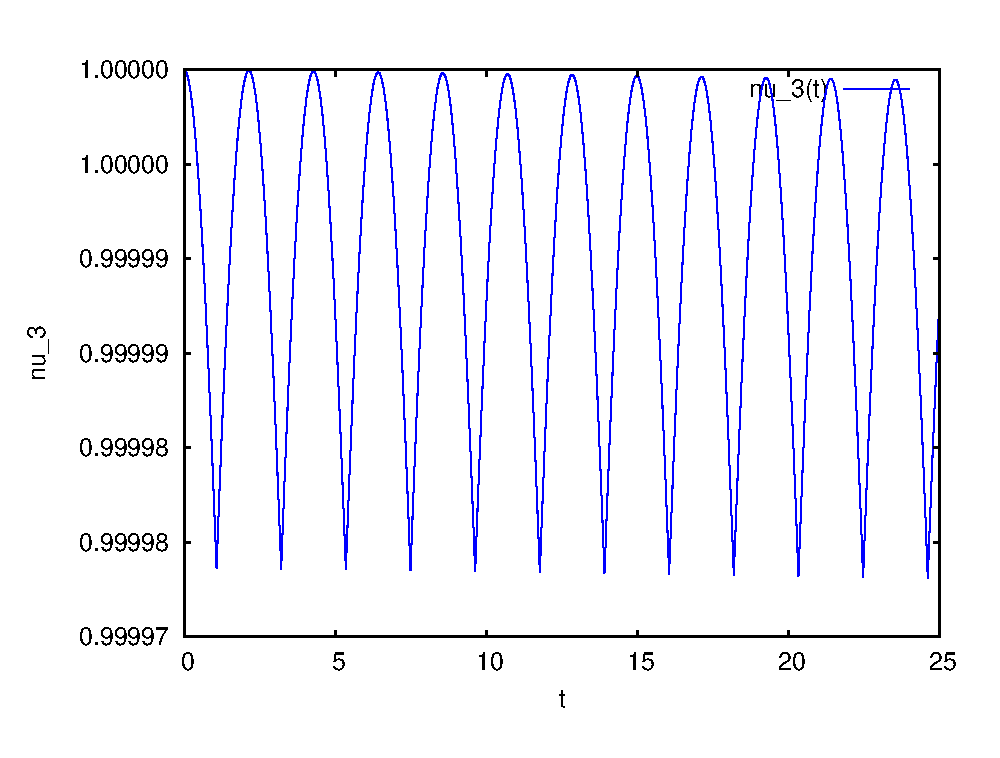
\includegraphics[width=\linewidth]{pic/rol__self_rot__velocity_of_self_rotation}
        \caption{Угловая скорость собственного вращения $\nu_3(t)$}
        \label{fig:rol__self_rot__velocity_of_self_rotation}    
    \end{subfigure}

    \caption{Экипаж с роликами. Вращение вокруг своей оси ($\nu_{1,2}(0) = 0, \nu_3 = 1$).}
    \label{fig:selfrot}
    
\end{figure}


%\begin{figure}[H]
    \centering

    \begin{columns}
        \column{0.45\textwidth}
            \centering
            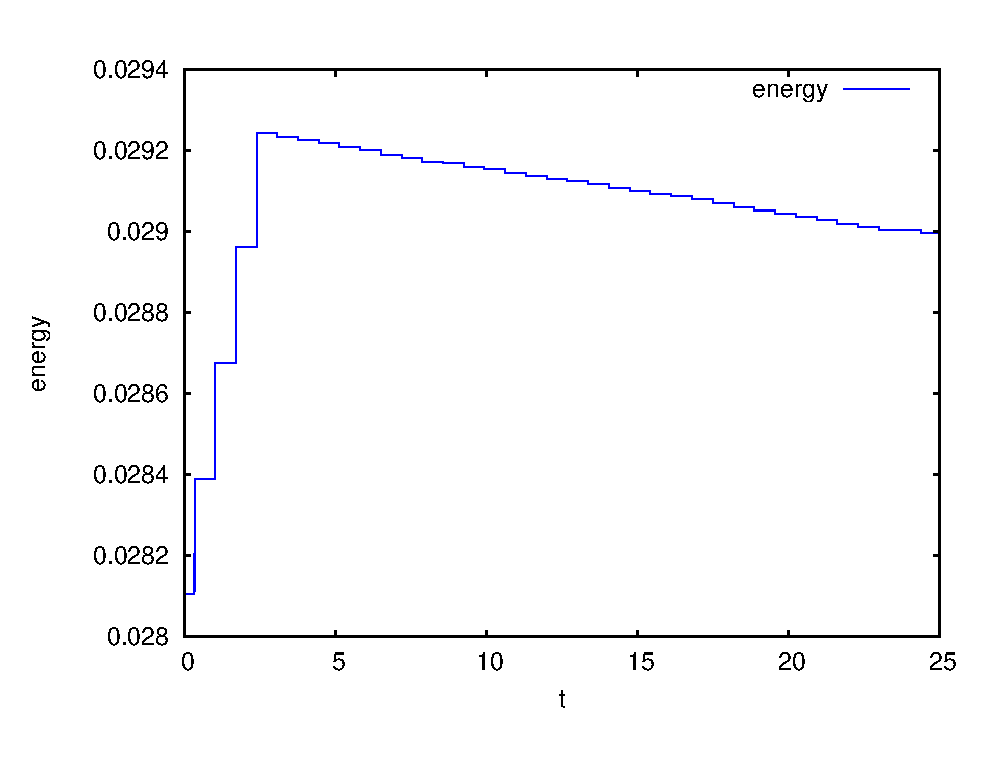
\includegraphics[width=\linewidth]{pic/rol__straight__kinetic_energy}\\
            Кинетическая энергия
        \column{0.45\textwidth}
            \centering
            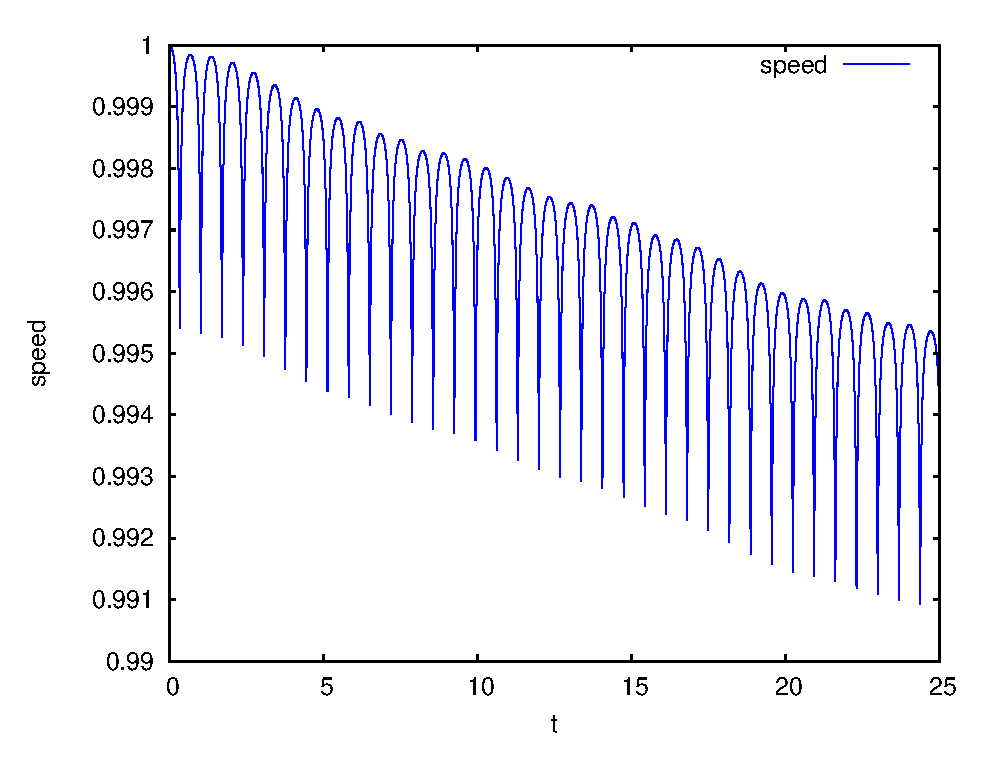
\includegraphics[width=\linewidth]{pic/rol__straight__speed_of_center_of_mass}\\
            Скорость центра масс
    \end{columns}
    
    \begin{columns}
        \column{0.35\textwidth}
            \centering
            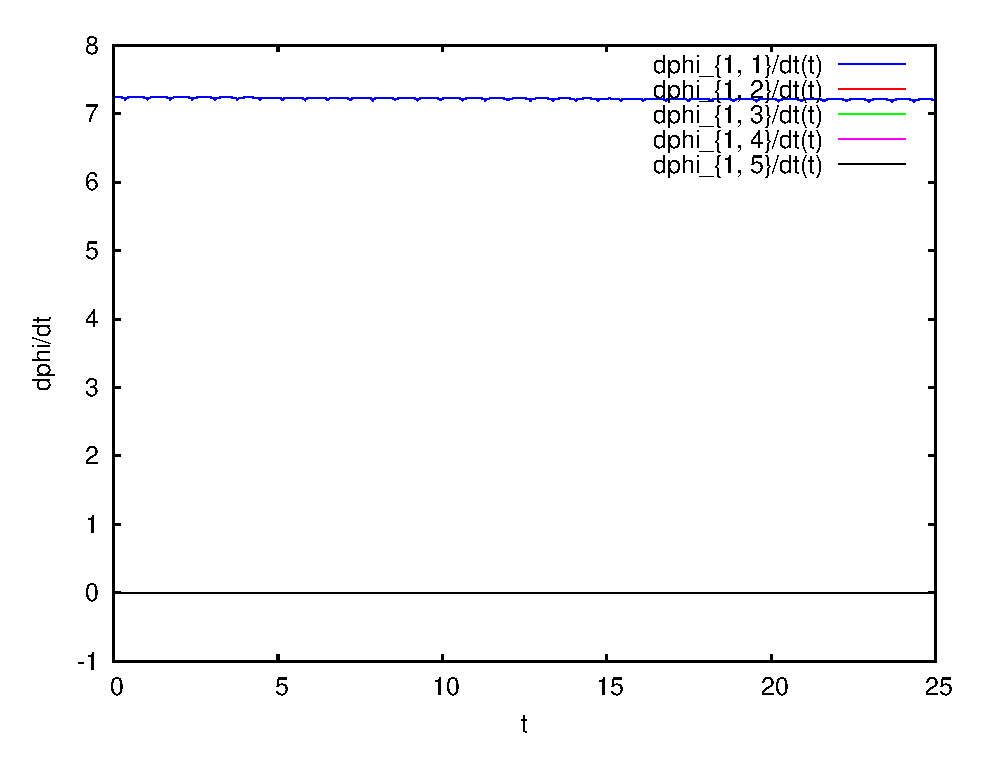
\includegraphics[width=\linewidth]{pic/rol__straight__velocities_of_rollers_of_wheel_1}\\
            $\dot{\phi}_{ij}(t)$ на переднем колесе
        \column{0.45\textwidth}
            \centering
            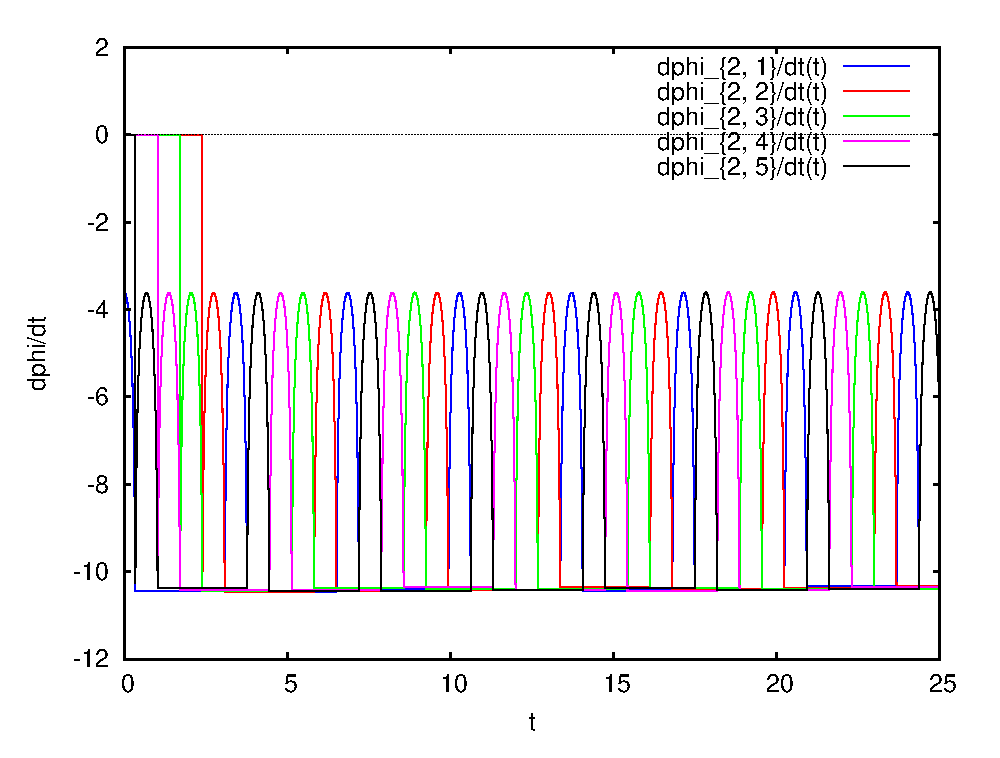
\includegraphics[width=\linewidth]{pic/rol__straight__velocities_of_rollers_of_wheel_2}\\
            $\dot{\phi}_{ij}(t)$ на правом заднем колесе
    \end{columns}

\end{figure}


%\begin{figure}
    \centering
    \begin{subfigure}[t]{0.45\textwidth}
        \centering
        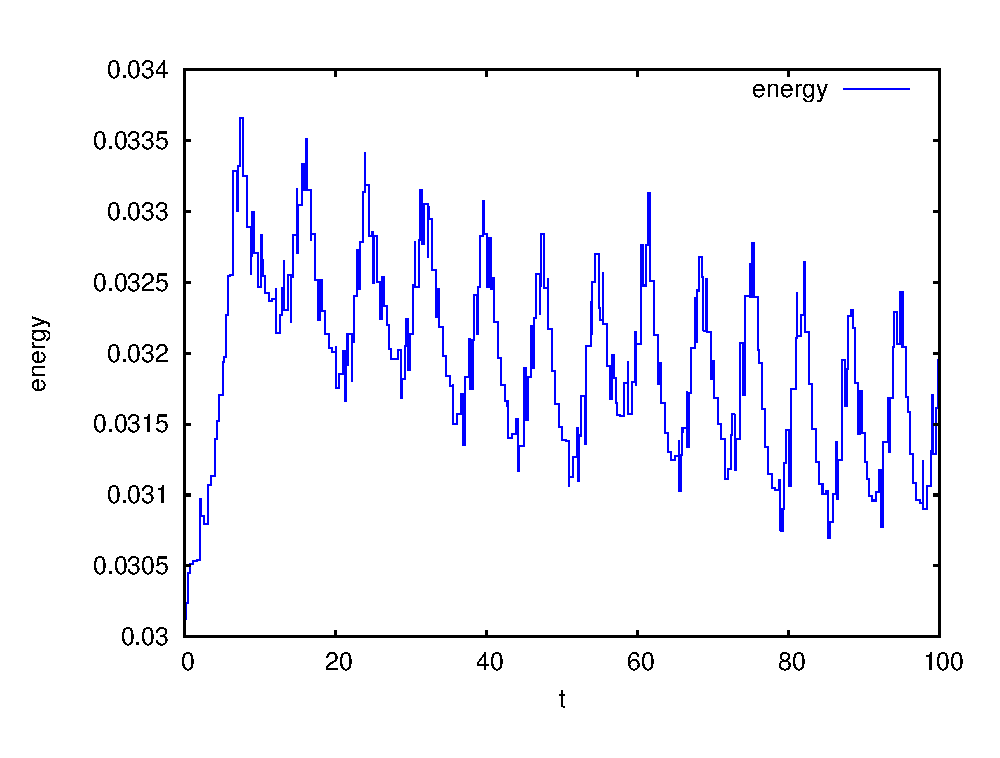
\includegraphics[width=\linewidth]{pic/rol__wrench__kinetic_energy}
        \caption{Кинетическая энергия}
        \label{fig:rol__wrench__kinetic_energy}
    \end{subfigure}
    \begin{subfigure}[t]{0.45\textwidth}
        \centering
        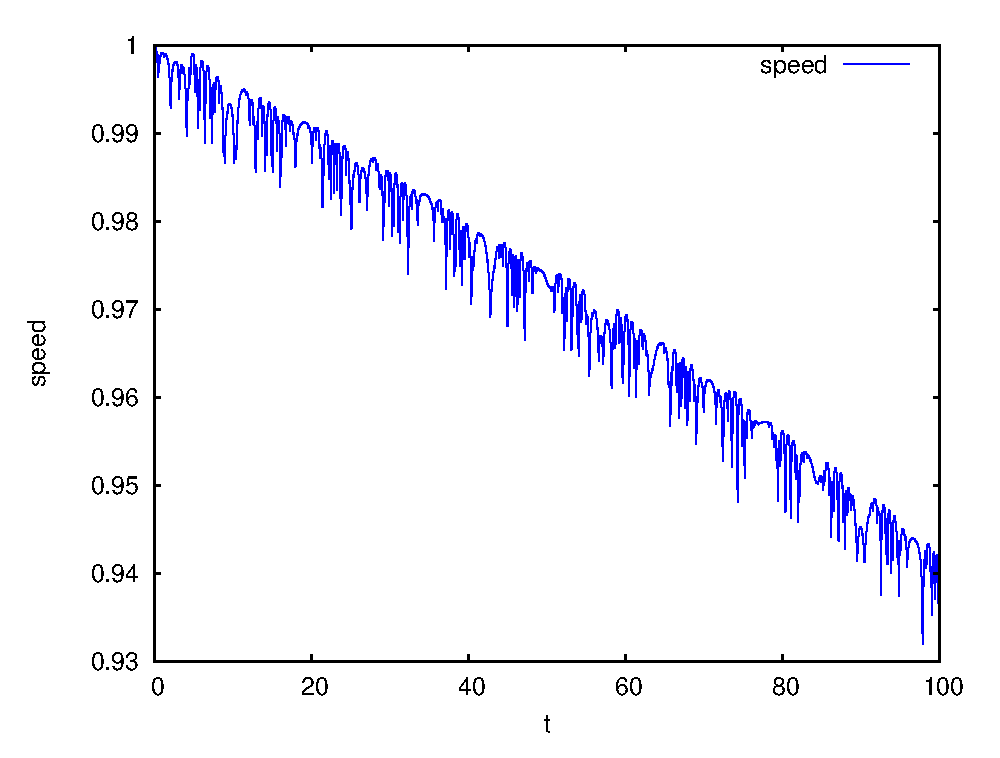
\includegraphics[width=\linewidth]{pic/rol__wrench__speed_of_center_of_mass}
        \caption{Скорость центра масс $\left(\nu_1^2 + \nu_2^2\right)(t)$}
        \label{fig:rol__wrench__speed_of_center_of_mass}
    \end{subfigure}
    \vspace{12pt}
    
    \begin{subfigure}[t]{0.45\textwidth}
        \centering
        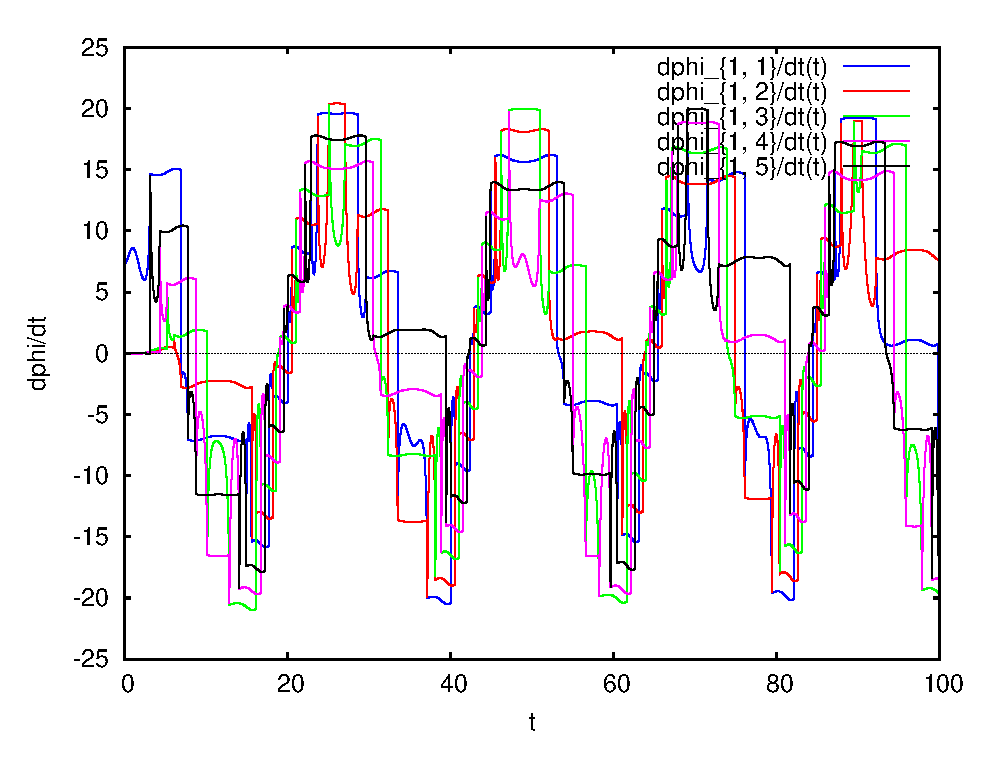
\includegraphics[width=\linewidth]{pic/rol__wrench__velocities_of_rollers_of_wheel_1}
        \caption{Скорости роликов $\dot{\phi}_{ij}(t)$ на первом колесе}
        \label{fig:rol__wrench__velocities_of_rollers_of_wheel_1}    
    \end{subfigure}
    \hfill
    \begin{subfigure}[t]{0.45\textwidth}
        \centering
        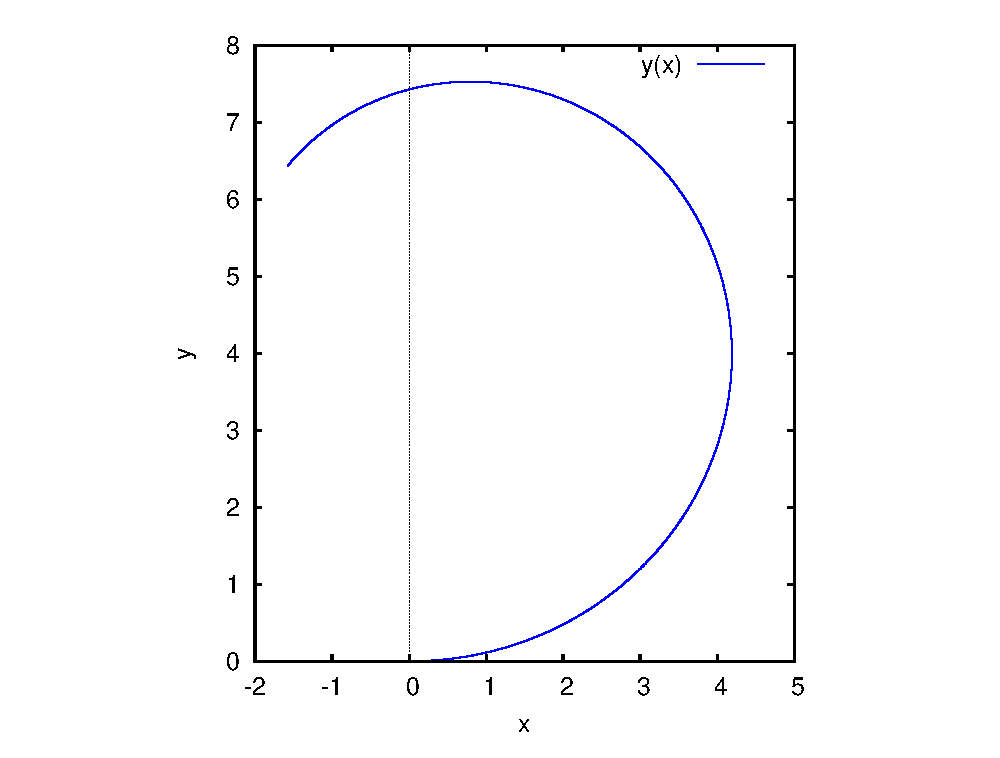
\includegraphics[width=\linewidth]{pic/rol__wrench__trajectory} \\
        \caption{Траектория центра масс на плоскости $OXY$}
        \label{fig:rol__wrench__trajectory}
    \end{subfigure}
    
    \caption{Экипаж c роликами. Движение с закруткой ($\nu_1(0) = 1, \nu_2(0) = 0, \nu_3(0) = 1$).}
    \label{fig:wrench}
    
\end{figure}
